% !TeX spellcheck = en_US
%\documentclass{beamer}
\documentclass[handout]{beamer}
\usepackage[spanish]{babel}
\usepackage[utf8]{inputenc}
\usepackage{graphicx}
\usepackage{tcolorbox}
\usepackage{color}
%\setbeamercolor{frametitle}{fg=white}
%\usefonttheme{structuresmallcapsserif}
\setbeamertemplate{footline}[frame number]
\setbeamerfont{footnote}{size=\tiny}

\setbeamercolor{page number in head/foot}{fg=black}

\usepackage{mhchem}
\usepackage{tikz}
\def\checkmark{\tikz\fill[scale=0.4](0,.35) -- (.25,0) -- (1,.7) -- (.25,.15) -- cycle;} 

\usepackage{default}

\usepackage[backend = bibtex, style = verbose, sorting = none, autocite = footnote]{biblatex}
\addbibresource{references.bib}

\newcommand\blfootnote[1]
{%
	\begingroup
	\renewcommand\thefootnote{}\footnote{#1}%
	\addtocounter{footnote}{-1}%
	\endgroup
}
\newcommand{\fcite}[1]{\blfootnote{\cite{#1}}}

\usetheme{Berkeley}

\begin{document}
	\begin{frame}
		\centering
		%\color{white}
		\textsc{\Large Start-up and calibration of a 2277 ThermoMetric calorimeter}
		\begin{center}
			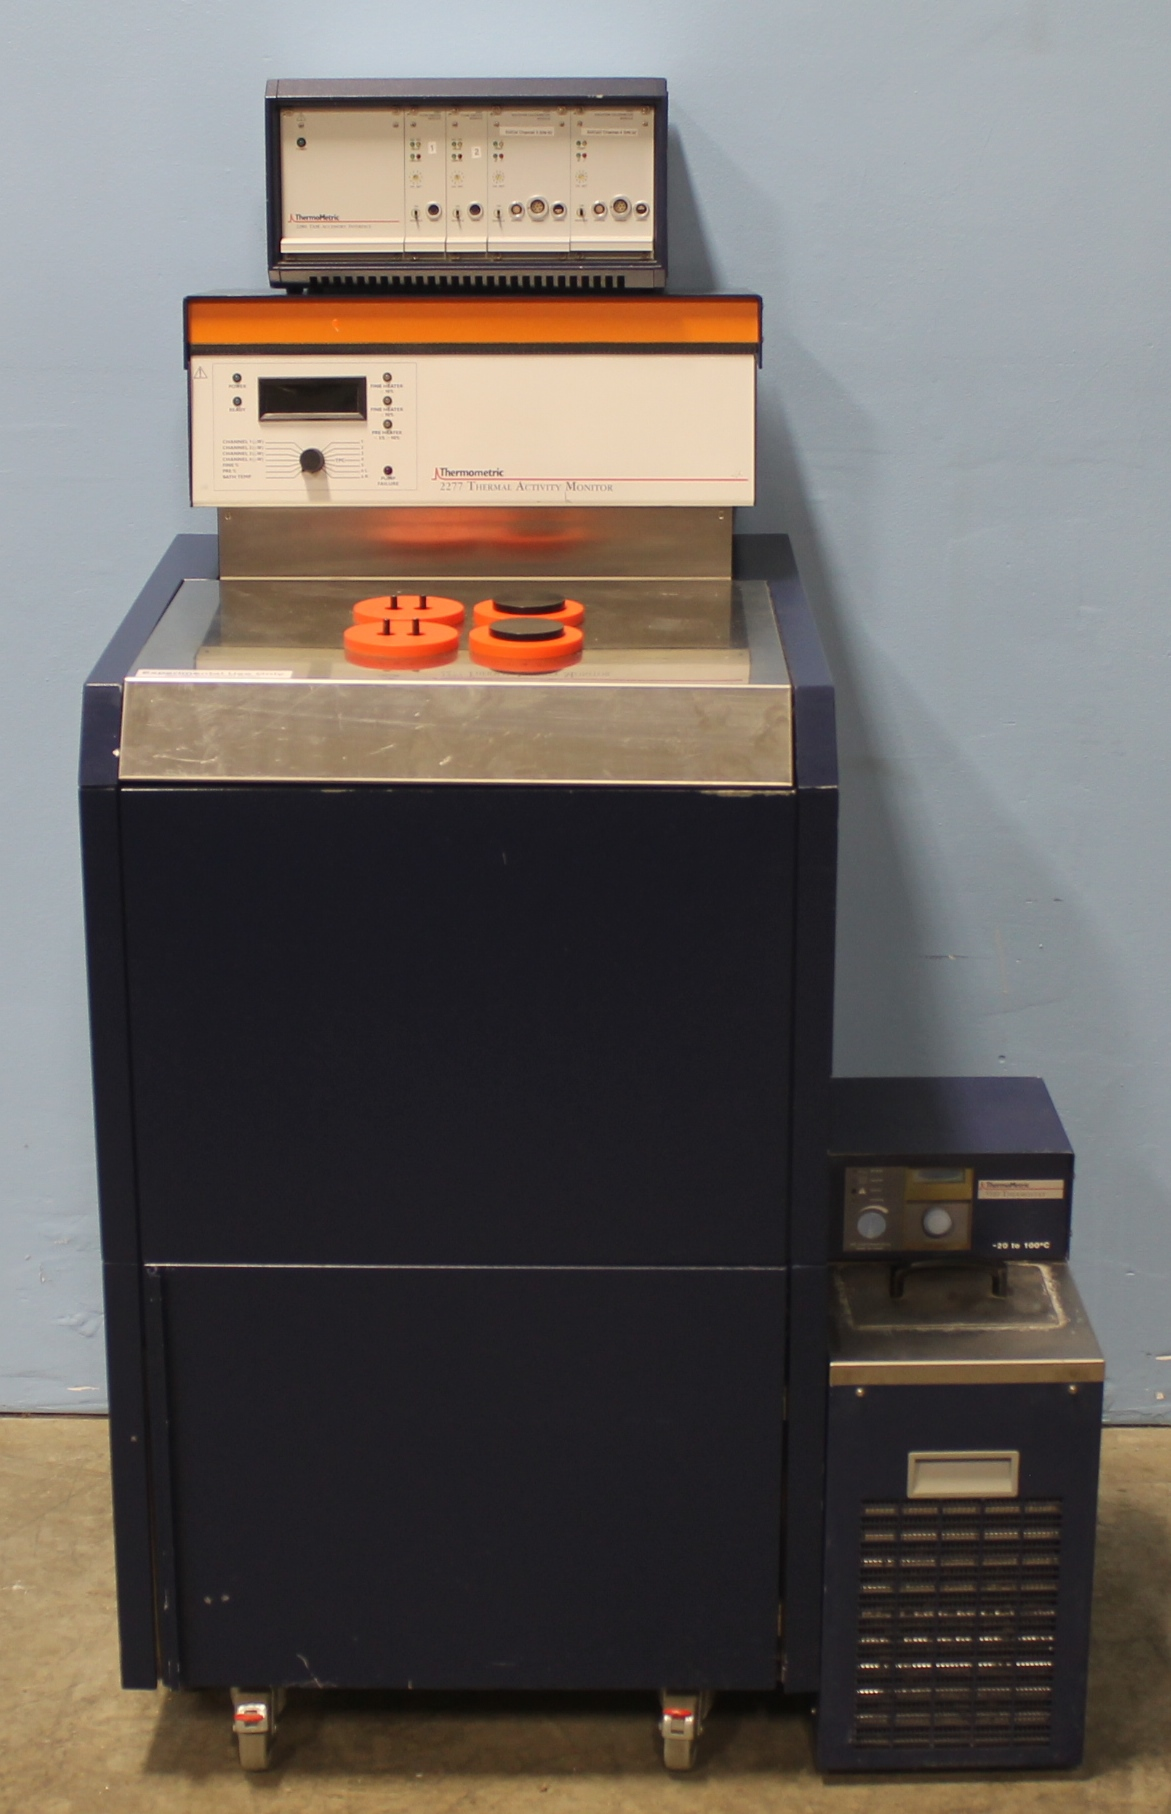
\includegraphics[width=0.3\linewidth]{sources/TAM}
		\end{center}
%		\\
		\vspace{0.2cm}
		\raggedleft \textbf{Presented by:} Juan Barbosa\\
		\raggedleft \textbf{Directed by:} Edgar Vargas, Dr. Sc.\\
		\raggedleft \textbf{Group:} Termodin\'amica de Soluciones
	\end{frame}

\begin{frame}{Contents}
	\tableofcontents
\end{frame}

\section{Introduction}
\begin{frame}{Introduction}
	\begin{table}[h]
		\centering
		\begin{tabular}{ccc}
			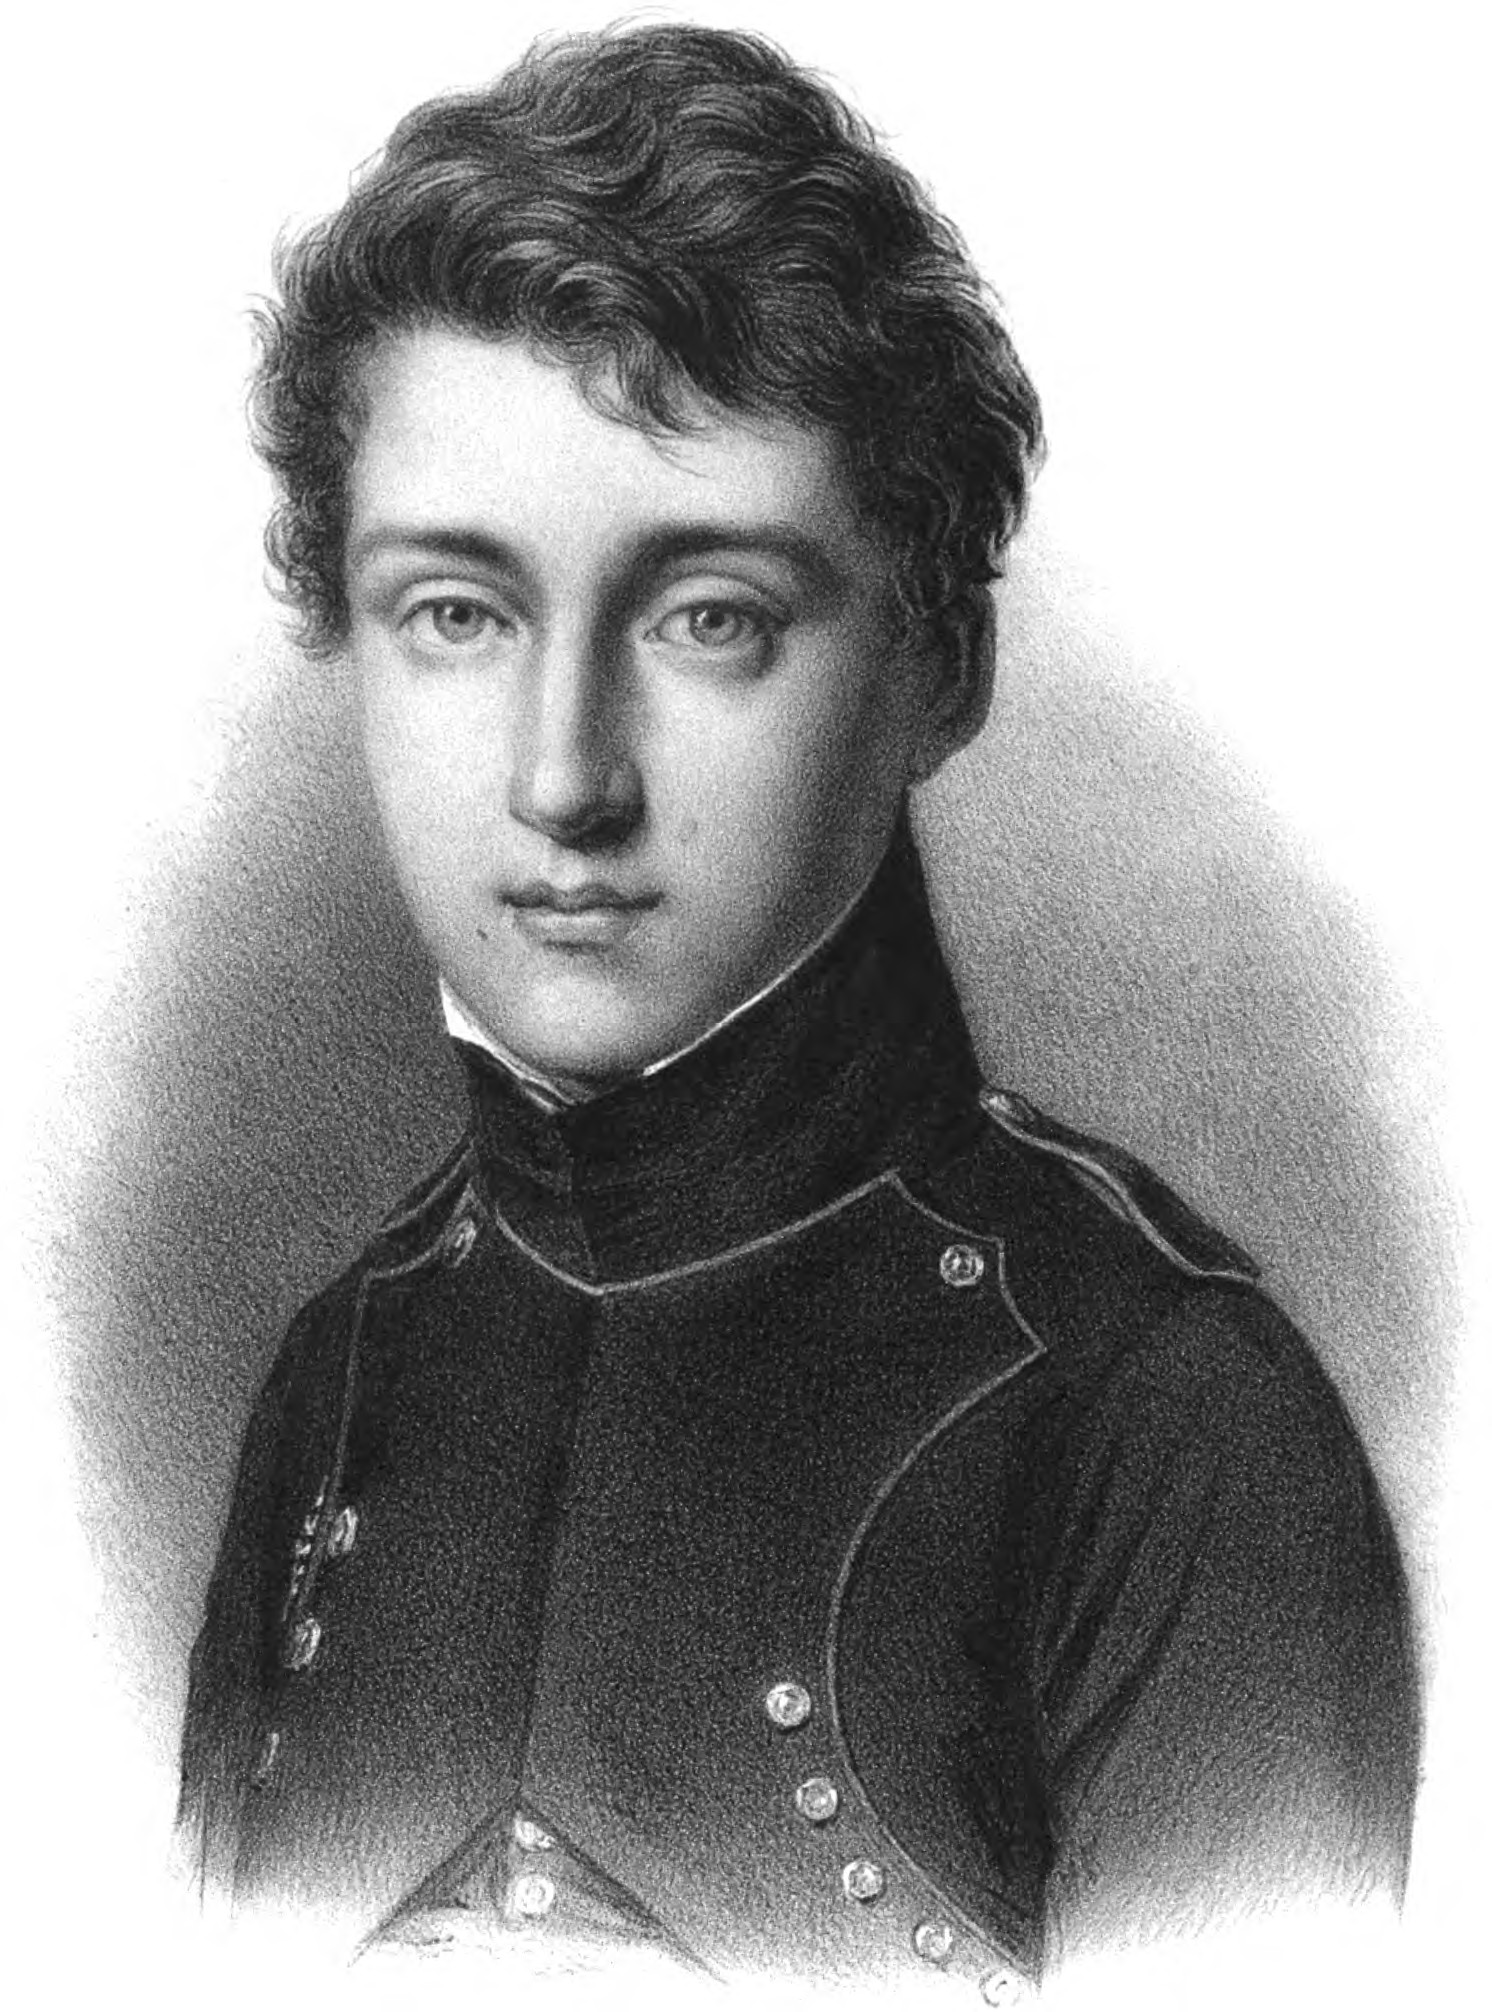
\includegraphics[width=0.25\linewidth]{sources/carnot} & 
			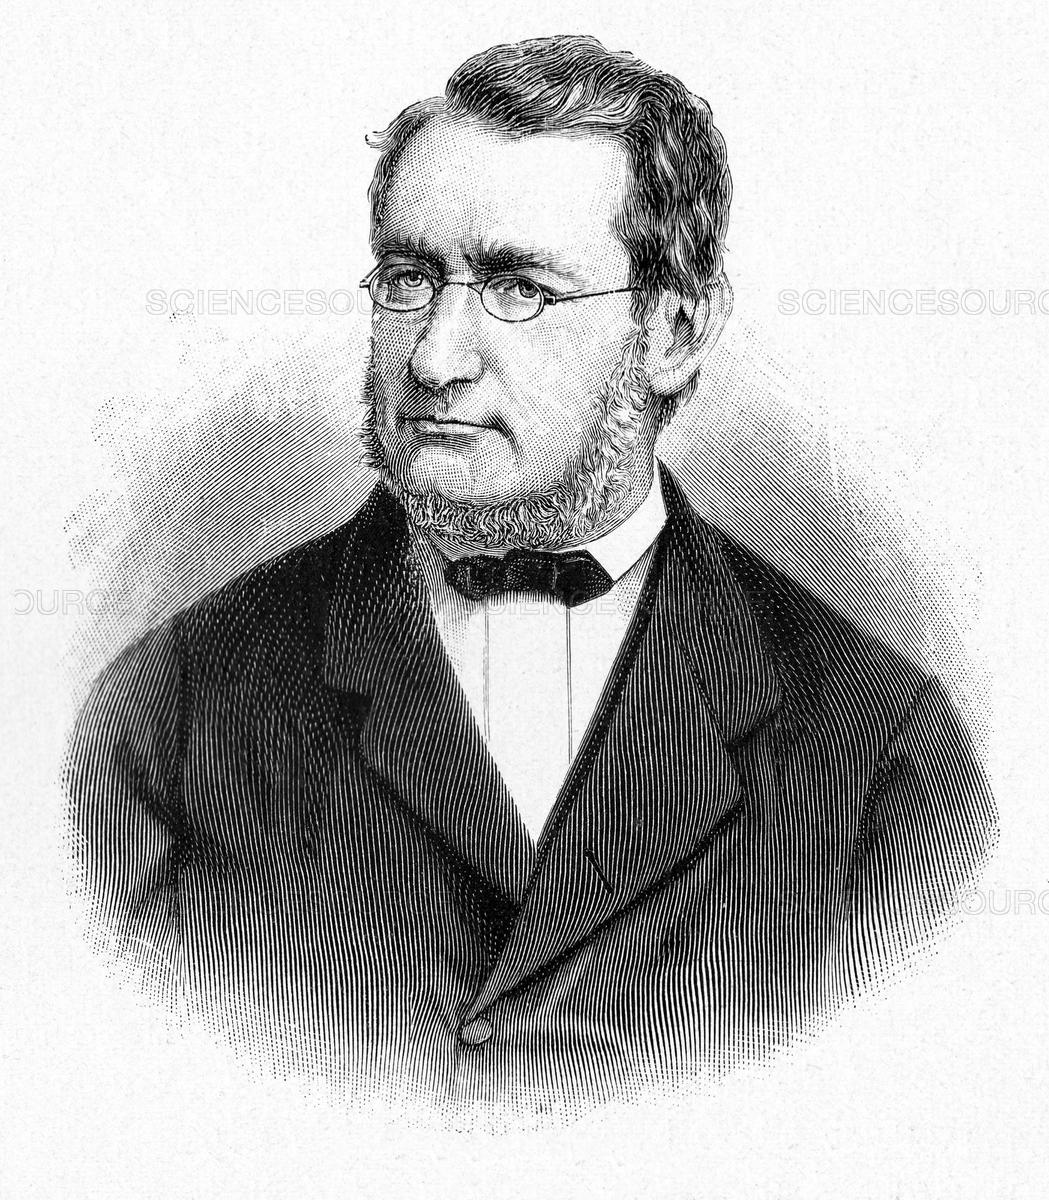
\includegraphics[width=0.25\linewidth]{sources/mayer} & 
			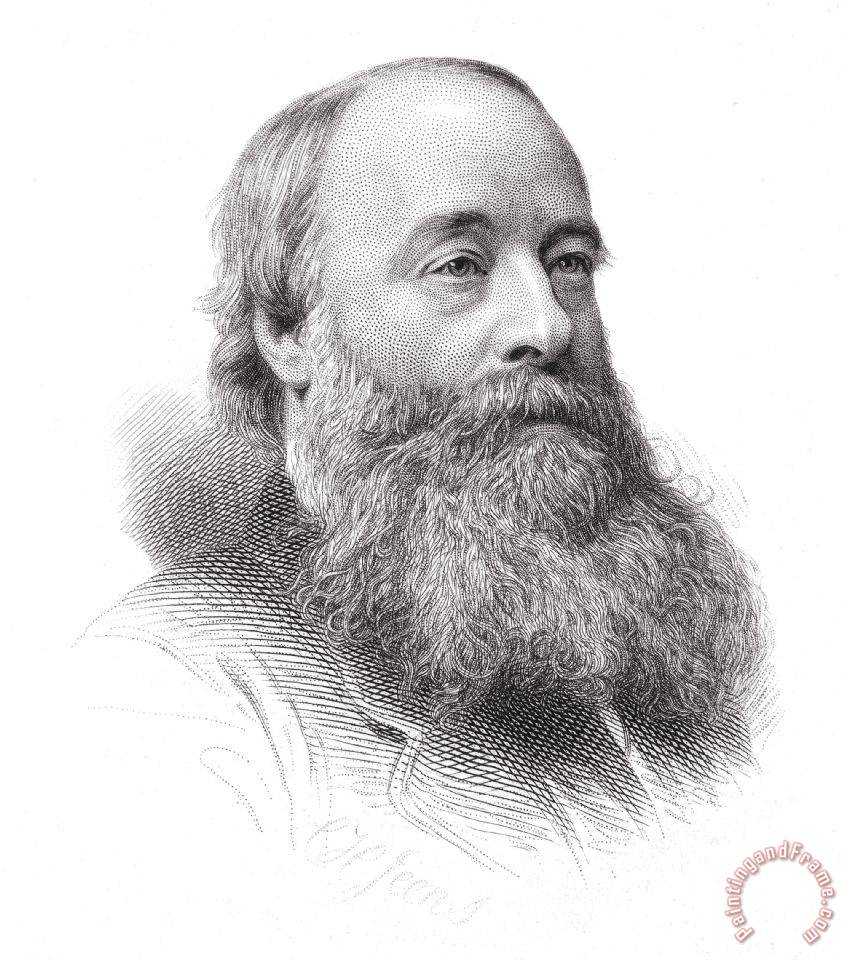
\includegraphics[width=0.25\linewidth]{sources/joule}\\
			Sadi Carnot & Julius von Mayer & James Joule	
		\end{tabular}
	\end{table}
	\begin{itemize}
		\item Thermodynamics is the study of energy transformations
		\item It was once thought that heat was a fluid
	\end{itemize}
	\fcite{feynman2011feynman}
	\fcite{fermi1986}
\end{frame}

\begin{frame}{Introduction}
	\begin{columns}
		\begin{column}{0.5\textwidth}
			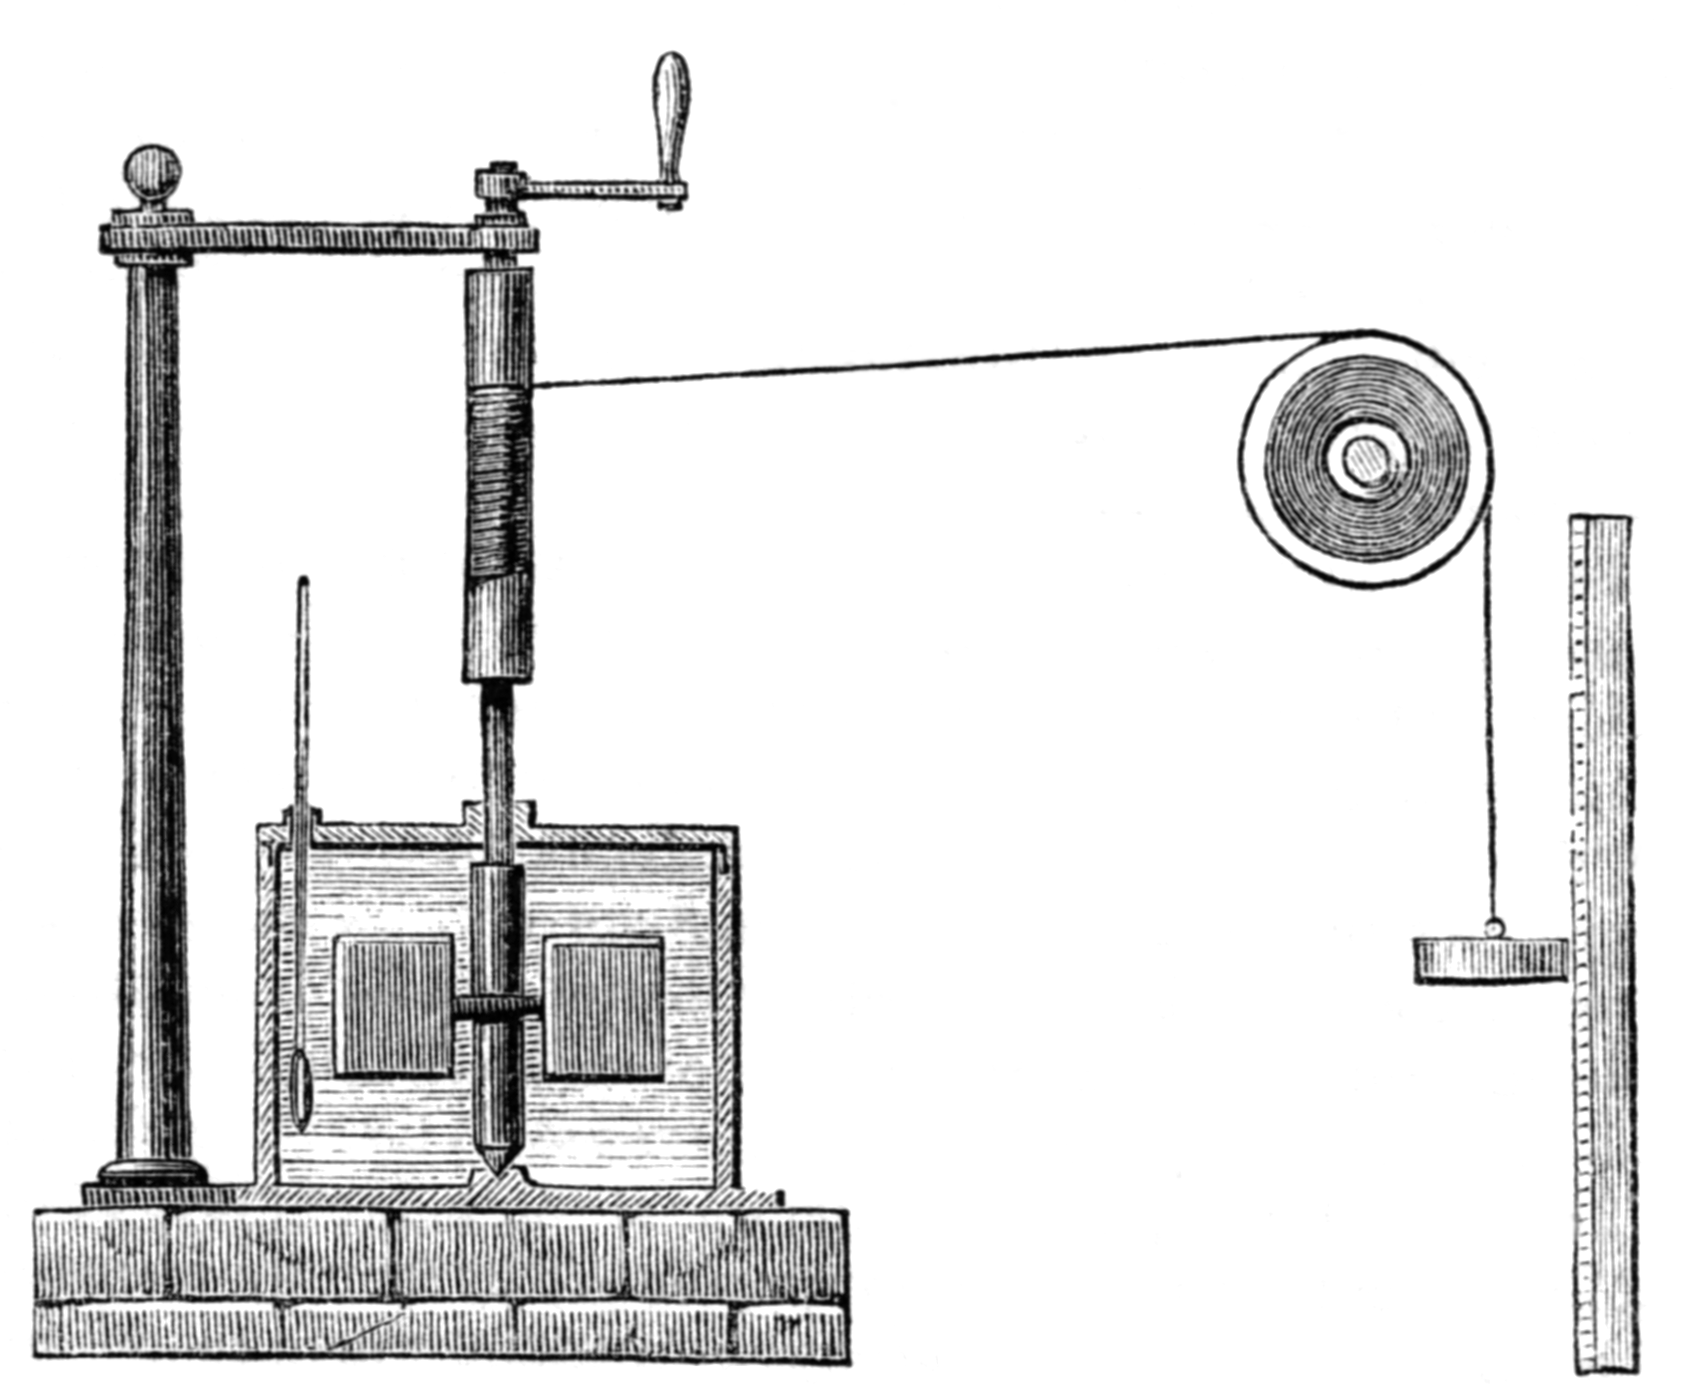
\includegraphics[width=\linewidth]{sources/joulesMachine}
		\end{column}
		\begin{column}{0.5\textwidth}
			\begin{itemize}
				\item $V = mgh$
				\item $T(V) = \dfrac{V}{m_{H_2O}C}$
			\end{itemize}
		\end{column}
	\end{columns}
	\begin{itemize}
		\item Heat is nowadays considered as a energy transfer.
	\end{itemize}
	\fcite{feynman2011feynman}
\end{frame}

\begin{frame}{Introduction}
	\begin{itemize}
		\item How is heat measured?\hspace{1cm} A \textbf{calorimeter}
		\item A Peltier element uses the Seebeck-Peltier effect to measure heat, and to transport it.
	\end{itemize}
	\begin{figure}[h]
		\centering
		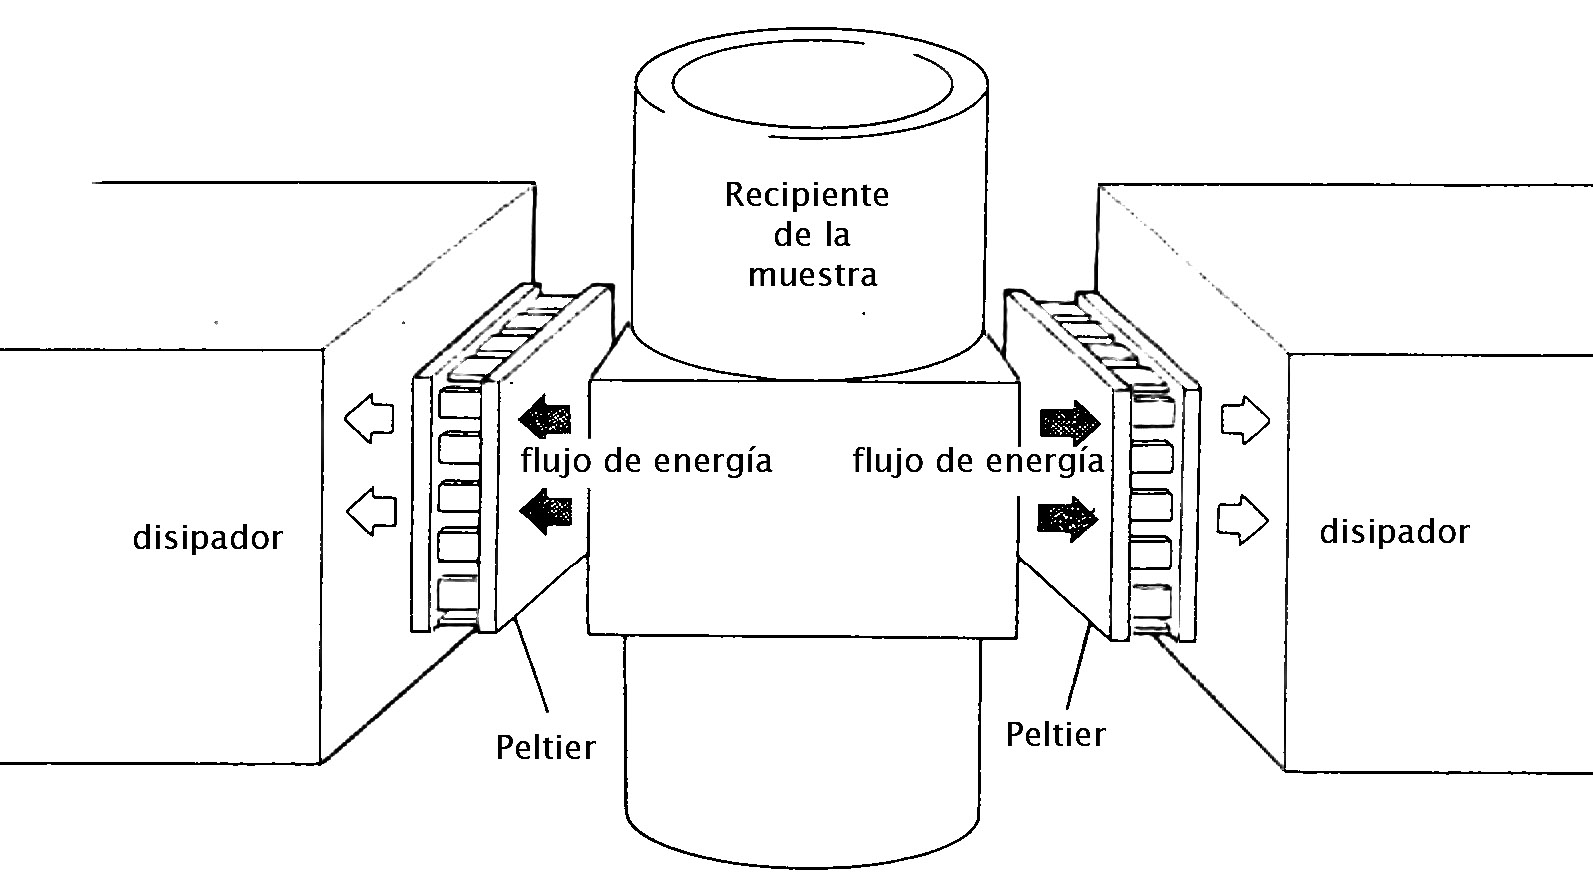
\includegraphics[width=0.8\linewidth]{sources/heatFlow}
	\end{figure}
	\begin{columns}
		\begin{column}{0.5\textwidth}
			\begin{equation}
				V = -S\nabla T \propto Q
			\end{equation}
		\end{column}
		\begin{column}{0.5\textwidth}
			\begin{equation}
				Q = \Pi I
			\end{equation}
		\end{column}
	\end{columns}
	\begin{equation}
		\Pi = TS
	\end{equation}
	\fcite{Suurkuusk}
\end{frame}

\section{Methodology}
\begin{frame}{Methodology}
	"Setup the 2277 Thermal Activity Monitor of the department, and additionally, calibrate the equipment for use in the active investigations of the Termodin\'amica de Soluciones group."
	\begin{enumerate}
		\item Carry out the wiring and electrical connections relevant for the operation of the equipment in Colombia.
		\item Controlling the calorimeter temperature.
		\item Do an electrical calibration of the calorimeter.
		\item Determine the molar enthalpy, Gibbs free energy, entropy, and equilibrium constant, of the complexation of the barium cation with 18-crown-6 ether.
	\end{enumerate}
\end{frame}

\begin{frame}{1-Wiring and electrical connections...}
	Out of the box
	\begin{tabular}{cc}
		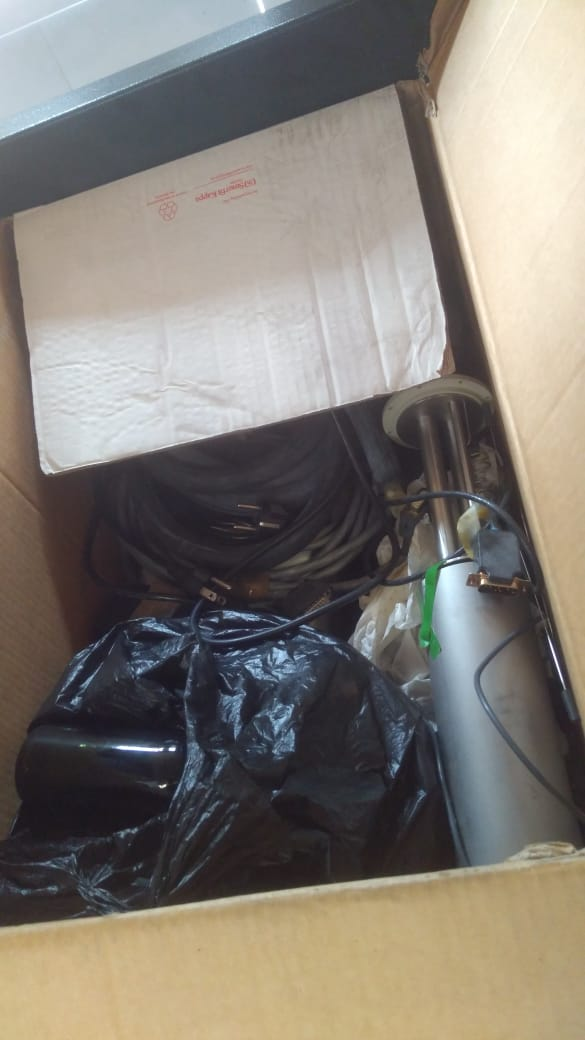
\includegraphics[width=0.2\linewidth]{sources/box1}
		& 
		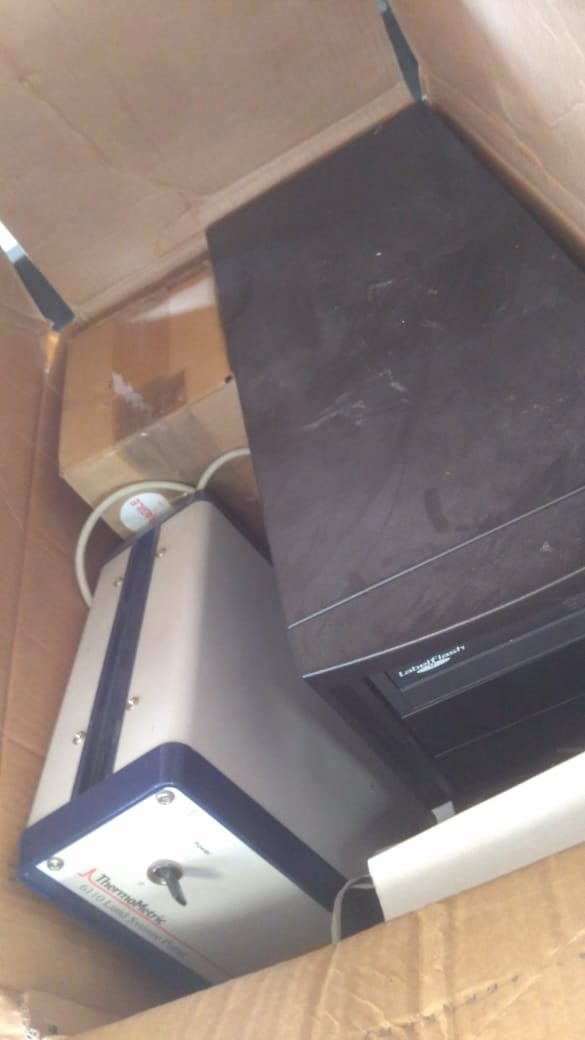
\includegraphics[width=0.2\linewidth]{sources/box2}
	\end{tabular}

	\begin{table}[h]
		\begin{tabular}{c}
			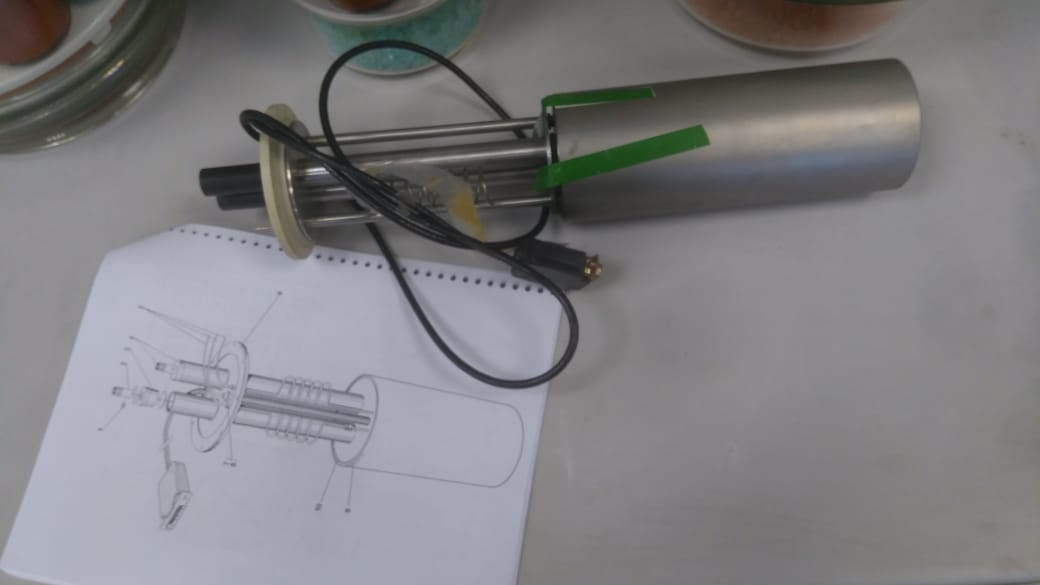
\includegraphics[width=0.6\linewidth]{sources/holder}
		\end{tabular}
	\end{table}
\end{frame}

\begin{frame}{1-Wiring and electrical connections...}
	\begin{table}[h]
		\begin{tabular}{cc}
			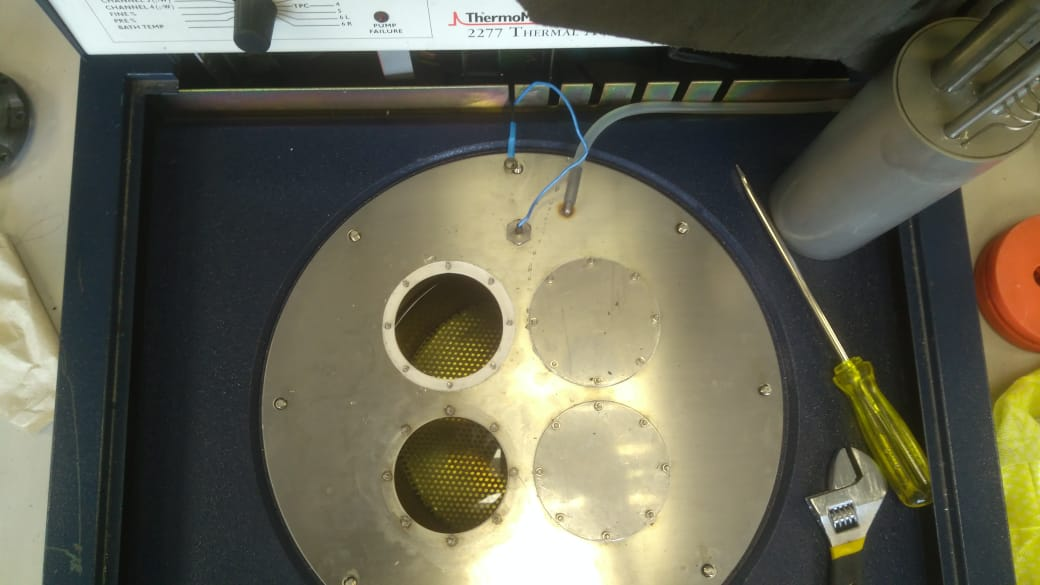
\includegraphics[width=0.4\linewidth]{sources/p1}
			& 
			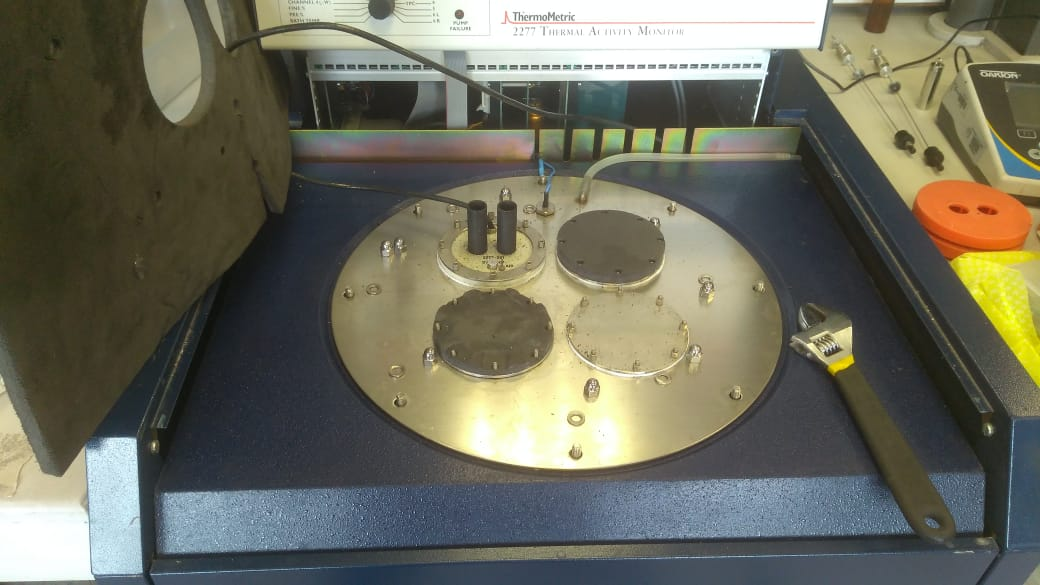
\includegraphics[width=0.4\linewidth]{sources/p2} \\
			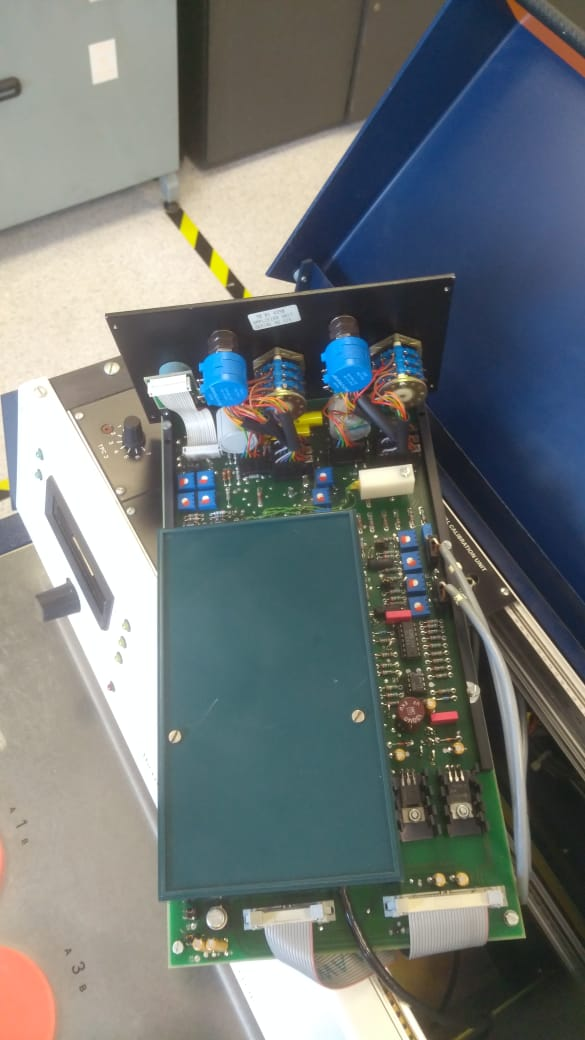
\includegraphics[width=0.25\linewidth]{sources/p3}
			& 
			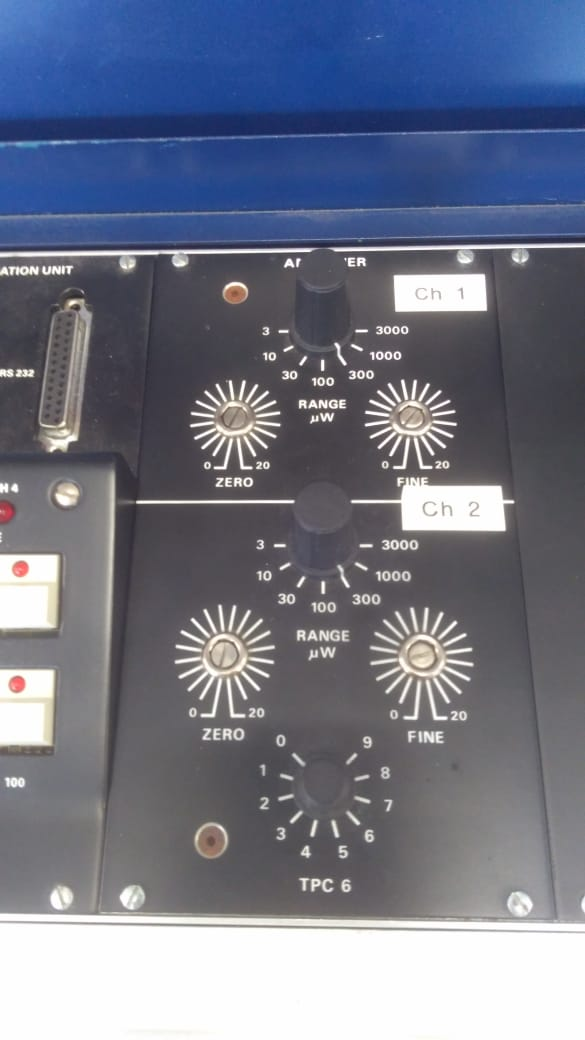
\includegraphics[width=0.25\linewidth]{sources/p4}
		\end{tabular}
	\end{table}
\end{frame}

\begin{frame}{1-Wiring and electrical connections...}
	\begin{columns}
		\begin{column}{0.7\textwidth}
			Power lines:
			\begin{itemize}
				\item \textbf{Sweden:} 220 VAC.
				\item \textbf{Colombia:} 110 VAC.
			\end{itemize}
			
			\begin{equation}
			P = VI = \dfrac{V^2}{R}
			\end{equation}
			
			Power must remain constant, that means doubling the current $\longrightarrow$ changing the fuses.
			
			\begin{figure}[h]
				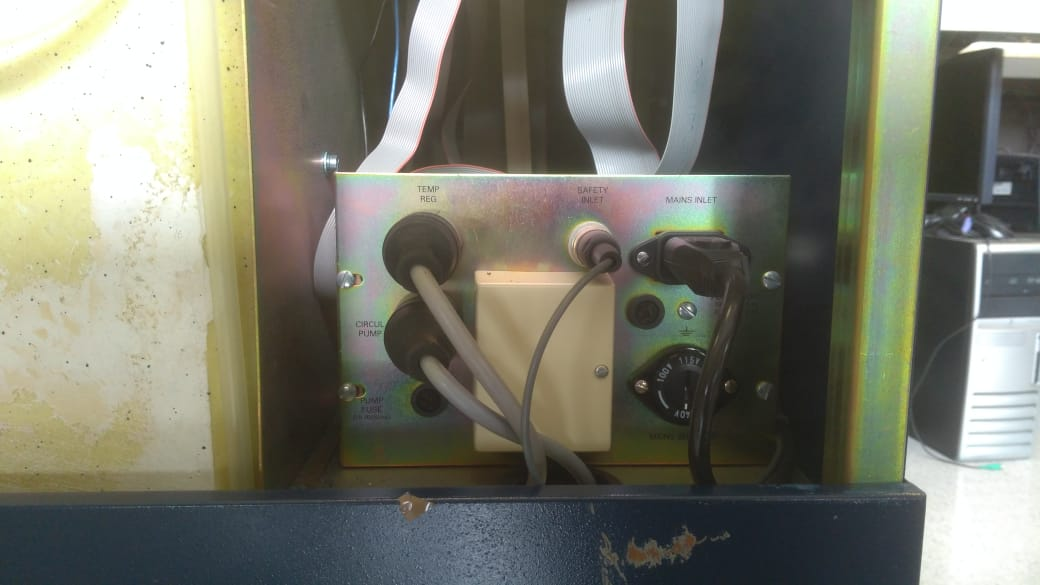
\includegraphics[width=.6\linewidth]{sources/f1}
			\end{figure}
		\end{column}
		\begin{column}{0.3\textwidth}
			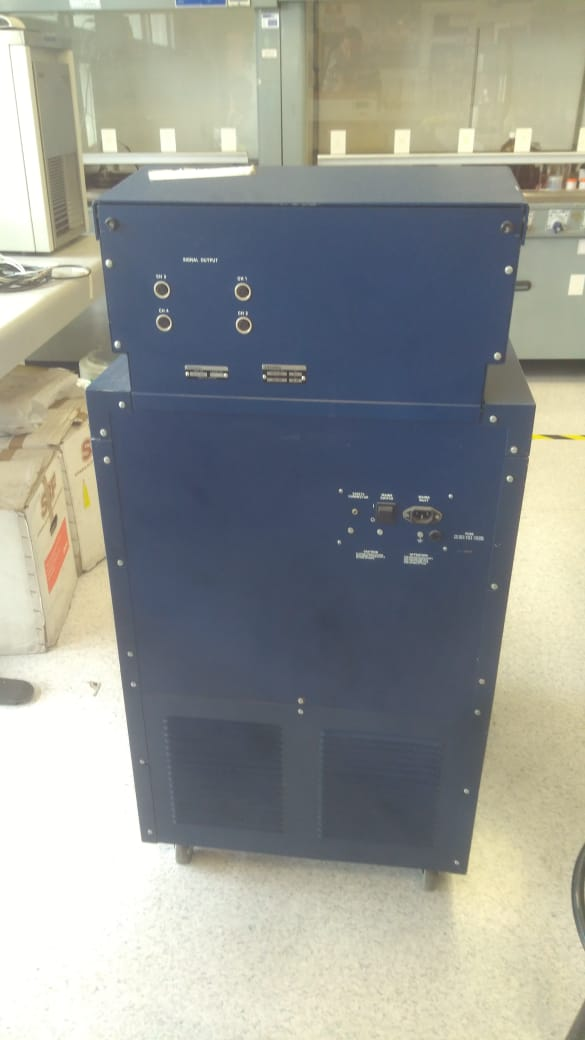
\includegraphics[width=\linewidth]{sources/f2}
		\end{column}
	\end{columns}
\end{frame}

\begin{frame}{2-Measuring temperature}
	\begin{columns}
		\begin{column}{0.65\textwidth}
			\begin{tabular}{c}
				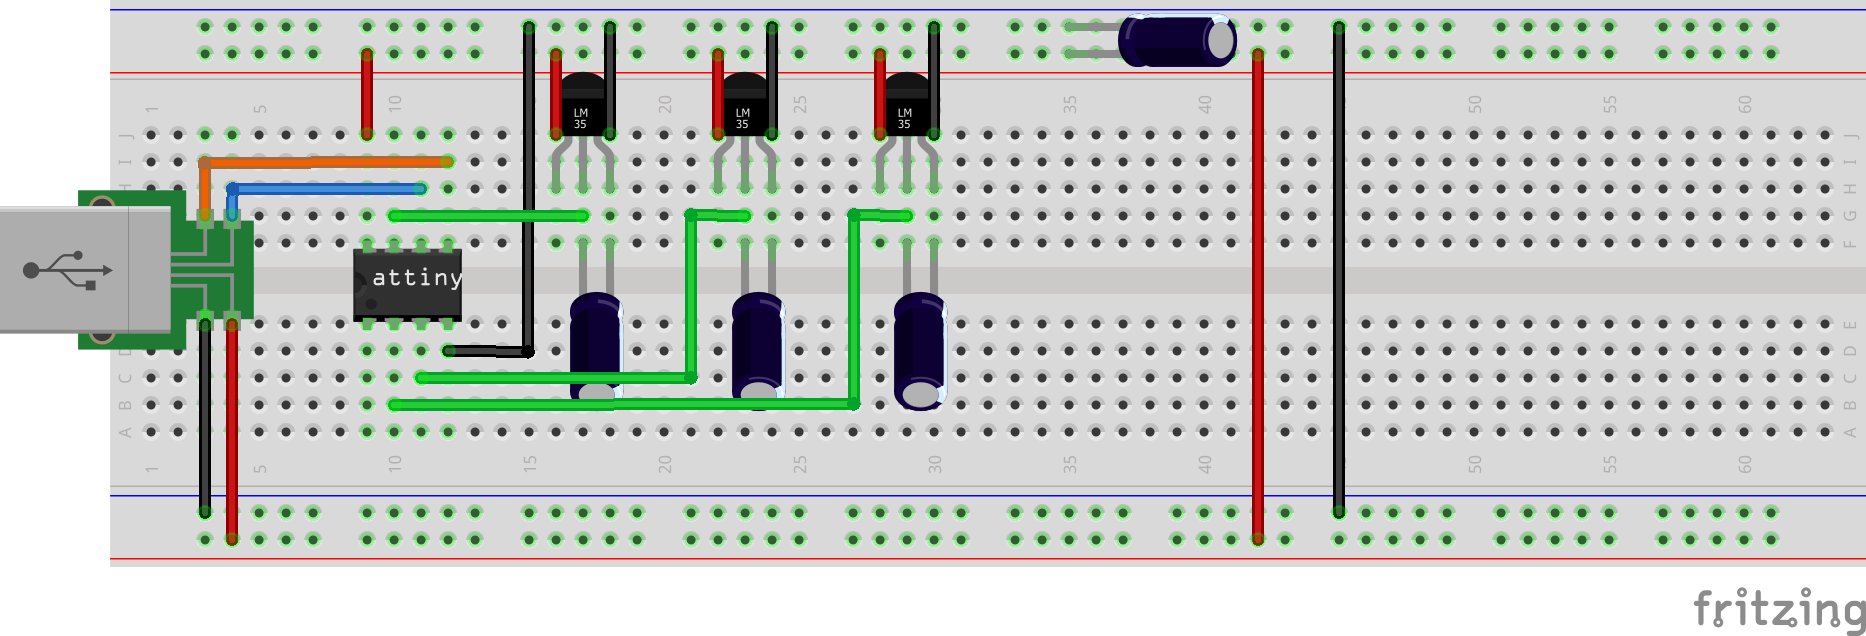
\includegraphics[width=\linewidth]{sources/Sketch_bb} \\
				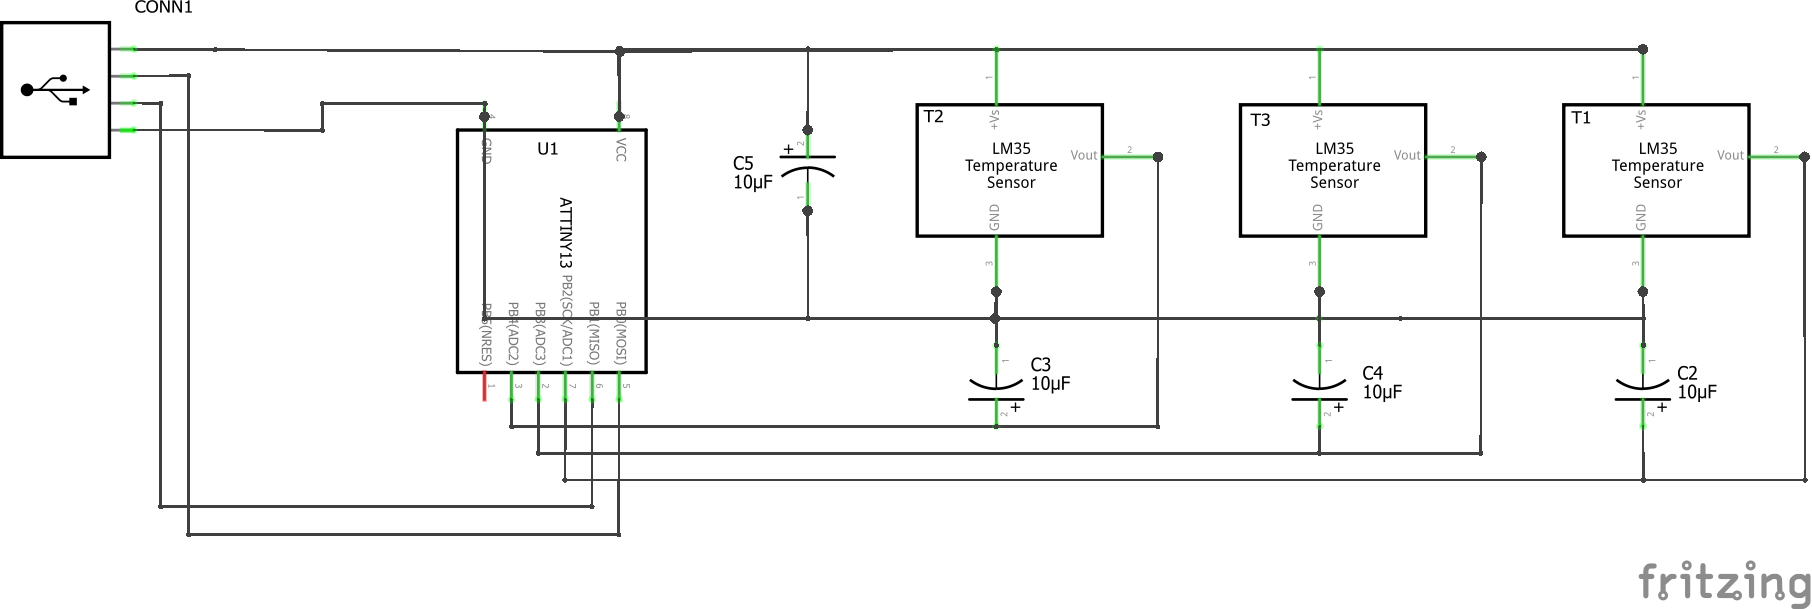
\includegraphics[width=\linewidth]{sources/Sketch_schem}
			\end{tabular}
		\end{column}
		\begin{column}{0.35\textwidth}
			\begin{tabular}{c}
				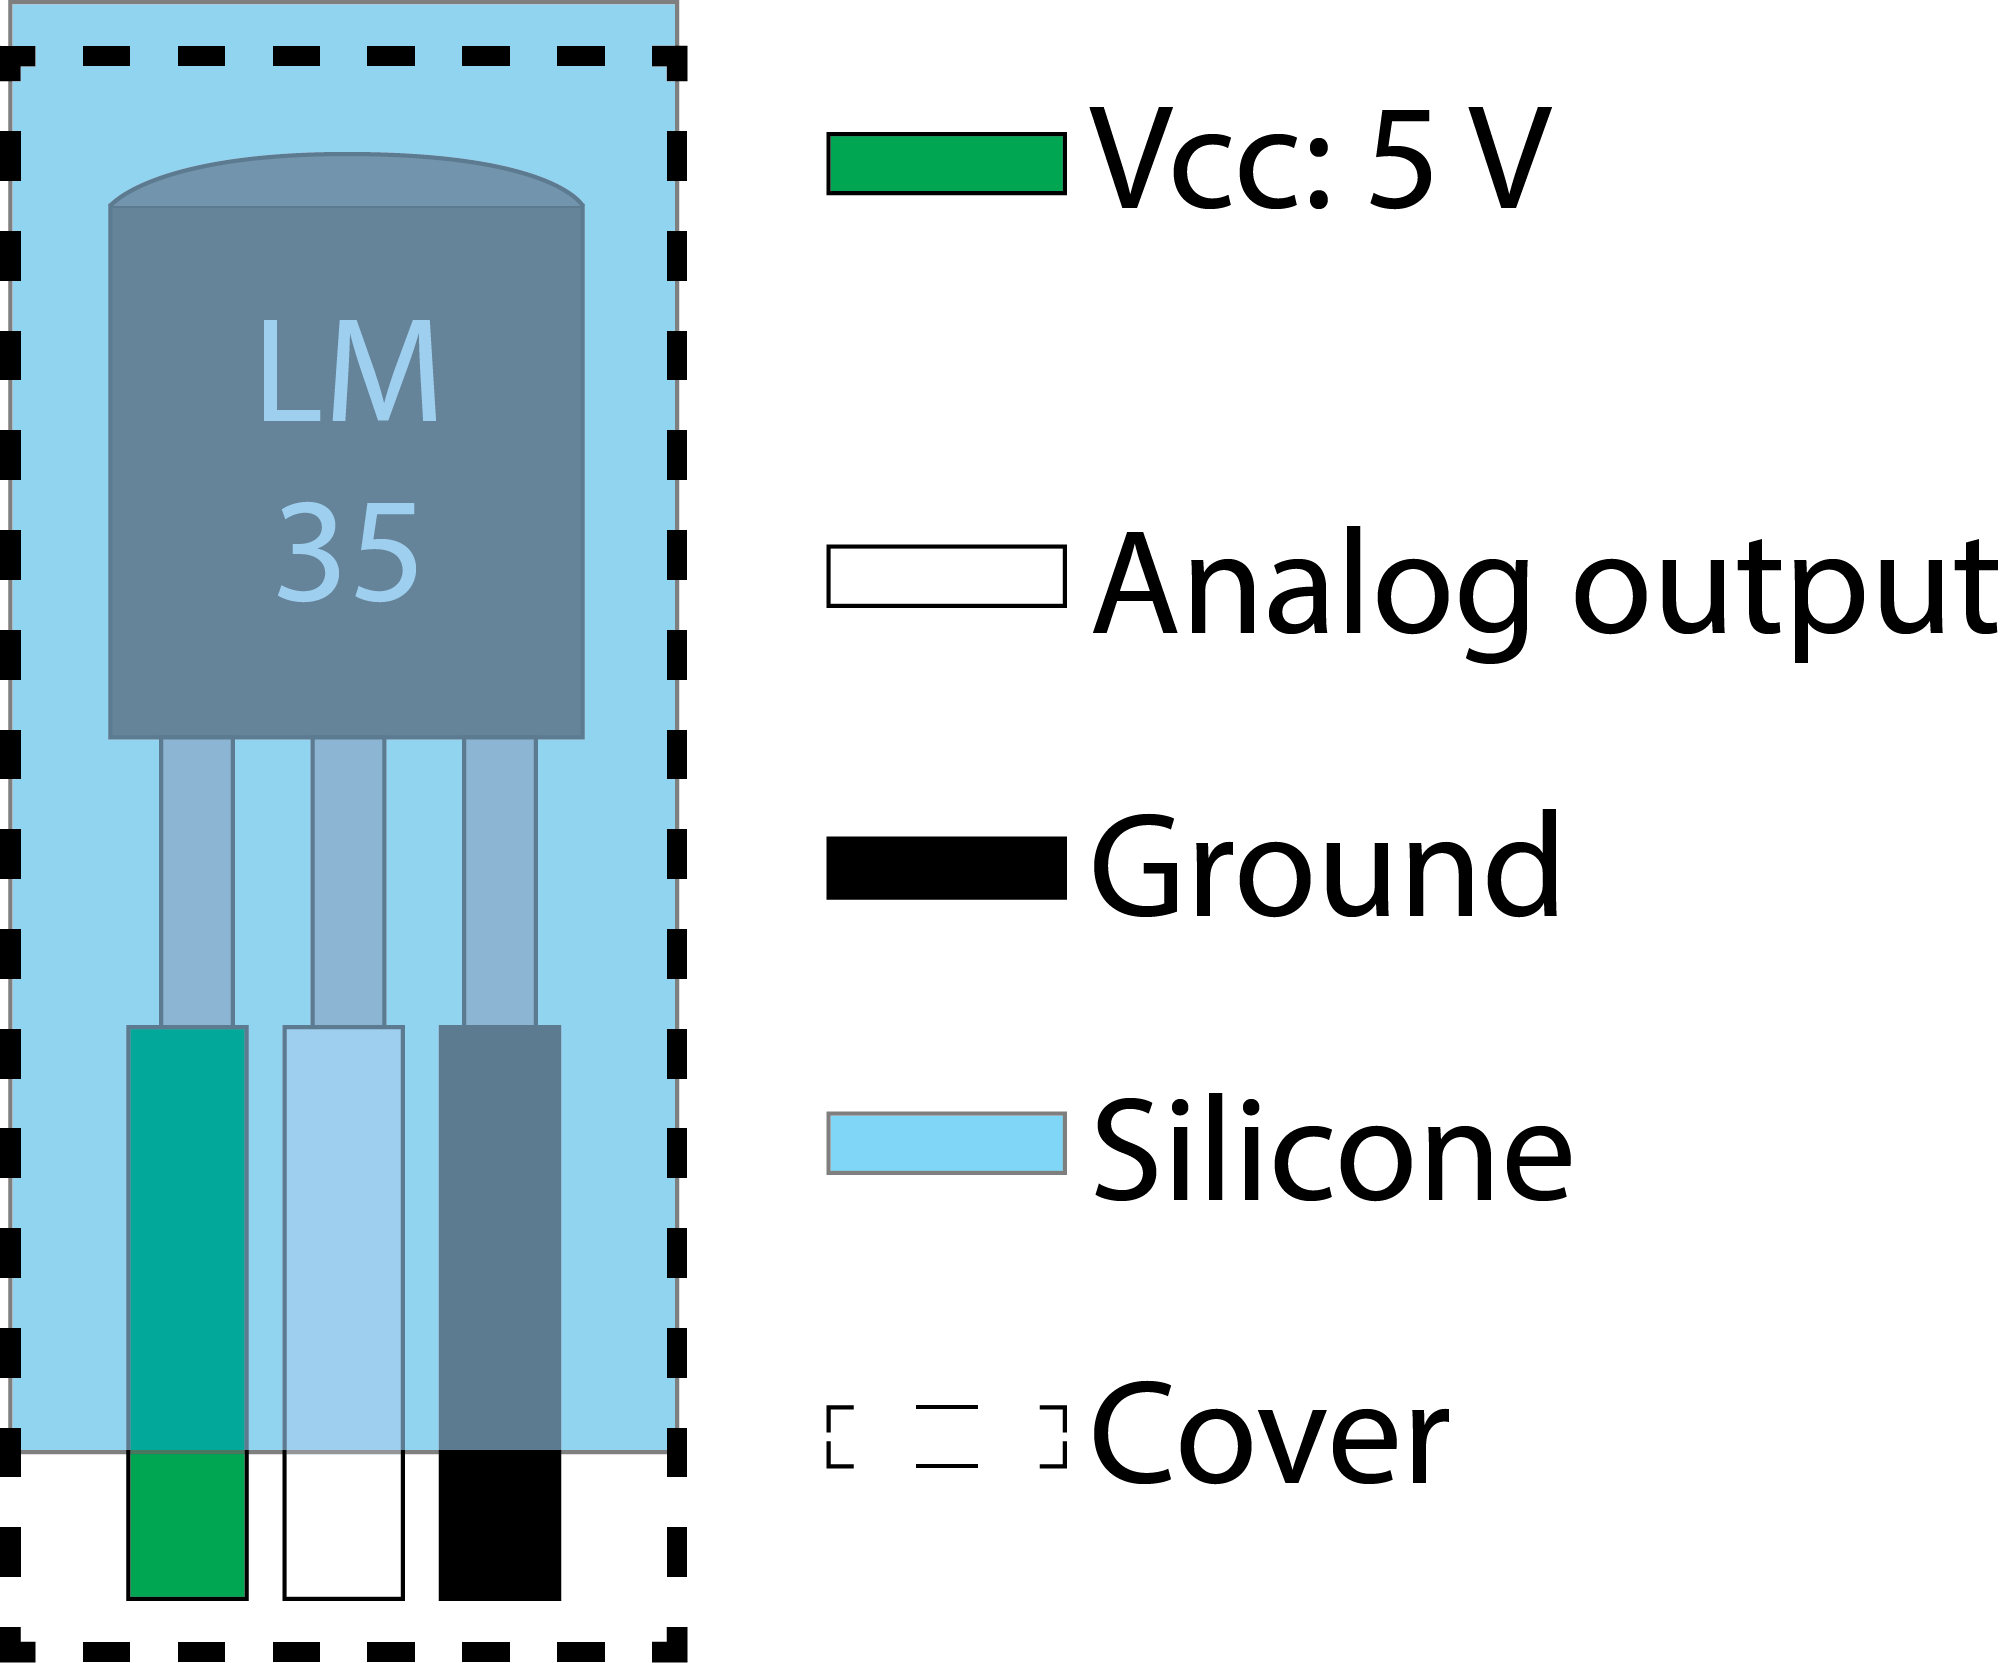
\includegraphics[width=\linewidth]{sources/Sensor} \\
				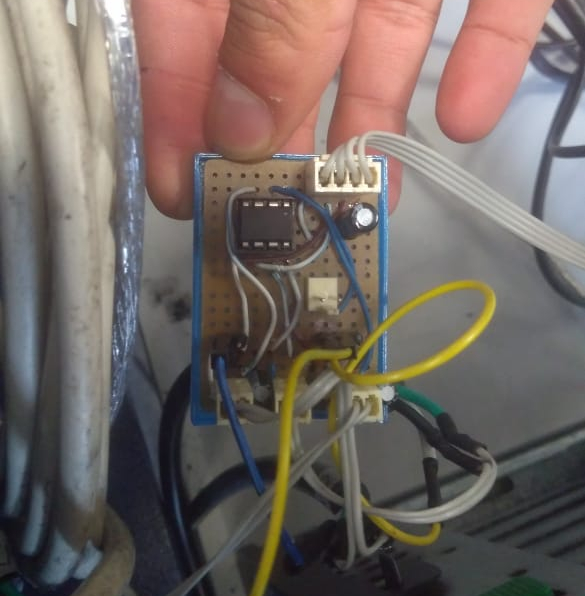
\includegraphics[width=0.8\linewidth]{sources/circuit}
			\end{tabular}
		\end{column}
	\end{columns}
\end{frame}

\begin{frame}{2-Measuring temperature}
	The small chip is called a Microcontroller.
	\begin{itemize}
		\item Firmware was written on C.
		\begin{itemize}
			\item An ADC is used to read an analog voltage.
			\item For a 0.01 $^\circ$C precision 10,000 different levels are needed (16 bits) $\longrightarrow$ oversampling.
			\item UART protocol for data communication.
		\end{itemize}
		\item Software on Python, real time temperature monitoring.
		
		\begin{table}[h]
			\begin{tabular}{cc}
				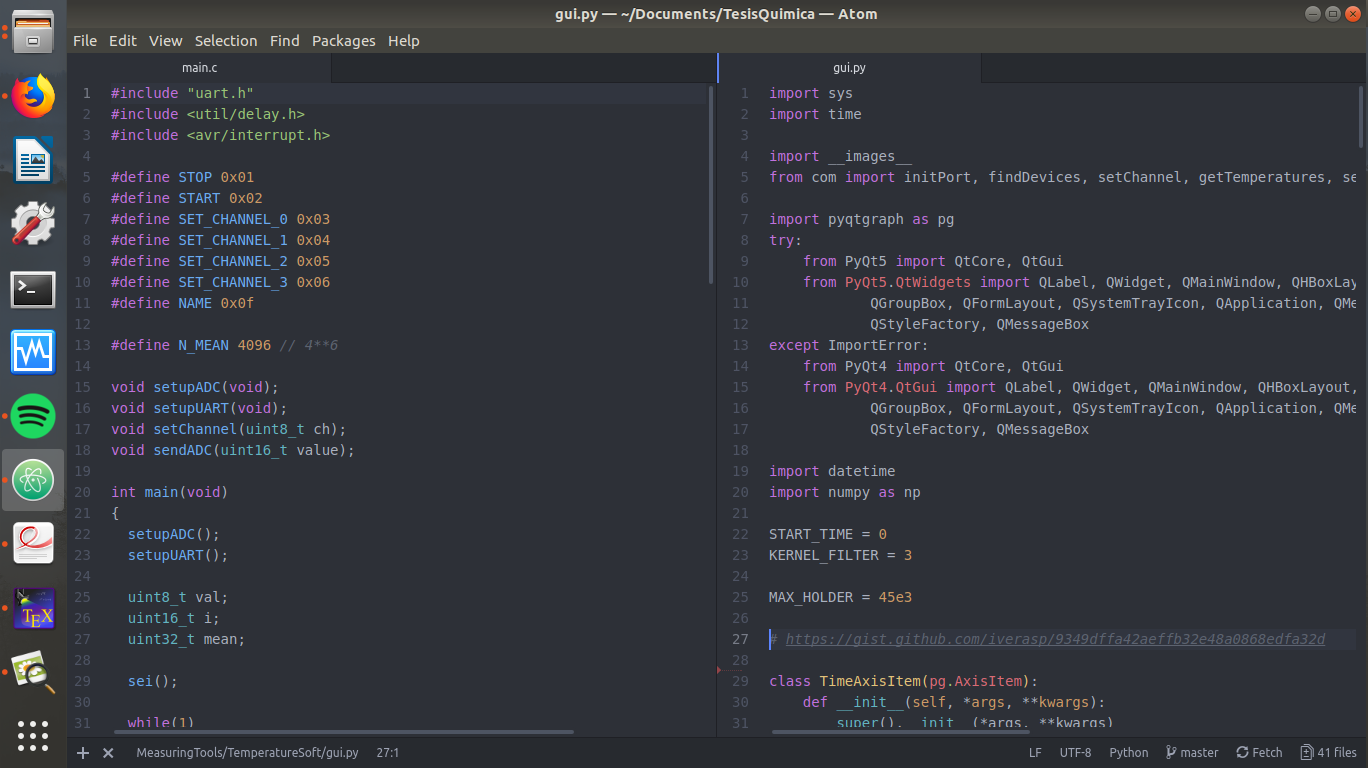
\includegraphics[width=0.45\linewidth]{sources/code} & 
				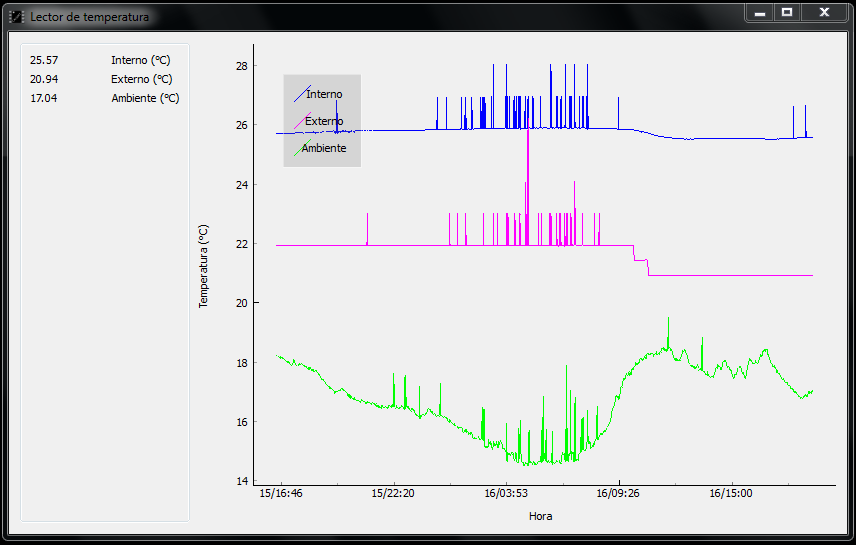
\includegraphics[width=0.4\linewidth]{sources/ss}
			\end{tabular}
		\end{table}
	\end{itemize} 
\end{frame}

\begin{frame}{2/3-Controlling temperature \& E. Calibration}
	\begin{itemize}
		\item Temperature control is done using 4, decade resistors.
		\begin{figure}[h]
			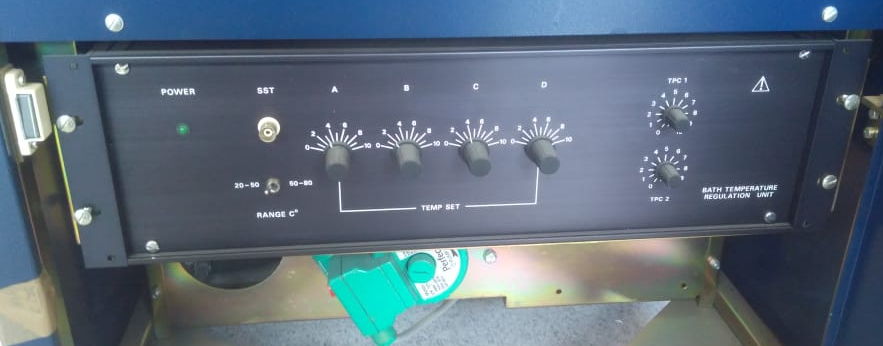
\includegraphics[width=0.5\linewidth]{sources/temperatureC}
		\end{figure}
		\item Electrical calibration is done using TM software, and controlling two, 10 turn potentiometers. $\longrightarrow$ A known 300 $\mu$W power is applied.
		\begin{figure}[h]
			\centering
			\begin{tabular}{cc}
				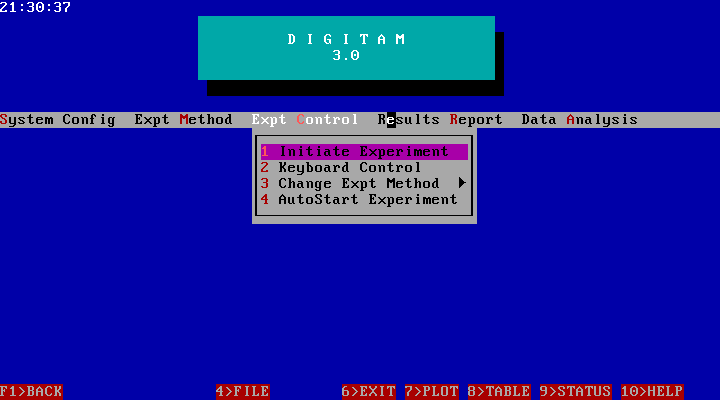
\includegraphics[width=0.5\linewidth]{sources/digitam} &
				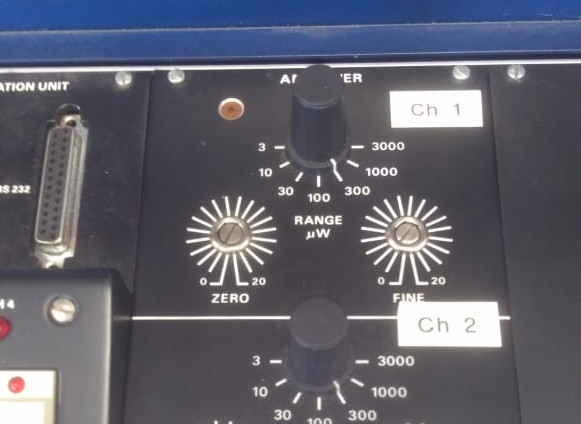
\includegraphics[width=0.38\linewidth]{sources/p5}
			\end{tabular}
		\end{figure}
	\end{itemize}
\end{frame}

\begin{frame}{4-Chemical calibration}
	\begin{itemize}
		\item Aqueous solutions of Barium chloride (\ce{BaCl2}) and 18-crown-6 ether (\ce{[C2H4O]6})
		\item Such solutions must be withing 1 mM and 10 mM for the ether, and 10 mM - 100 mM for the chloride. \fcite{mizoue2004calorimetric}
	\end{itemize}

	\begin{equation}
		\ce{Ba^{2+}(ac) + [C2H4O]6(ac) -> Ba^{2+}.[C2H4O]6(ac)}
	\end{equation}
	\begin{figure}[h]
		\centering
		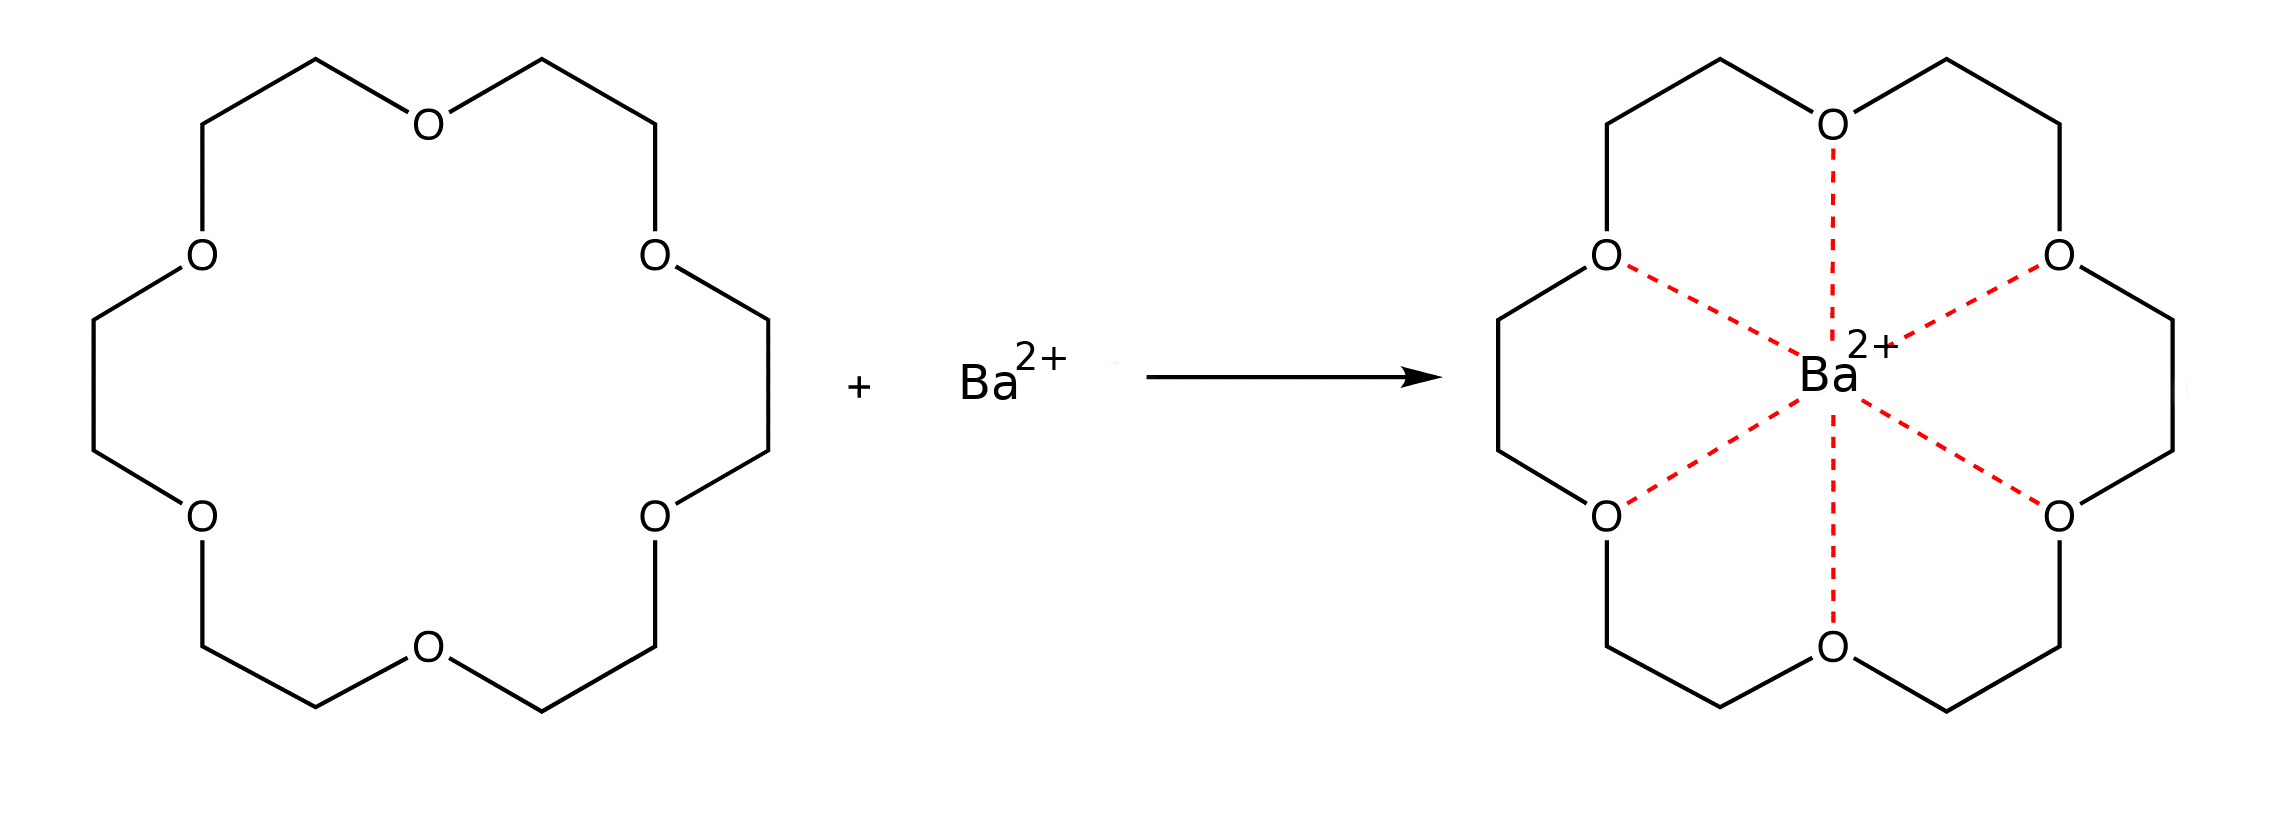
\includegraphics[width=0.6\linewidth]{sources/reaction}
	\end{figure}
	
\end{frame}

\begin{frame}{4-Chemical calibration}
	\begin{equation}
		\Delta H = Q + V\Delta P = Q
	\end{equation}
	\begin{equation}
		\Delta G = -RT\ln K_D = \Delta H - T\Delta S
	\end{equation}
	\begin{figure}[h]
		\centering
		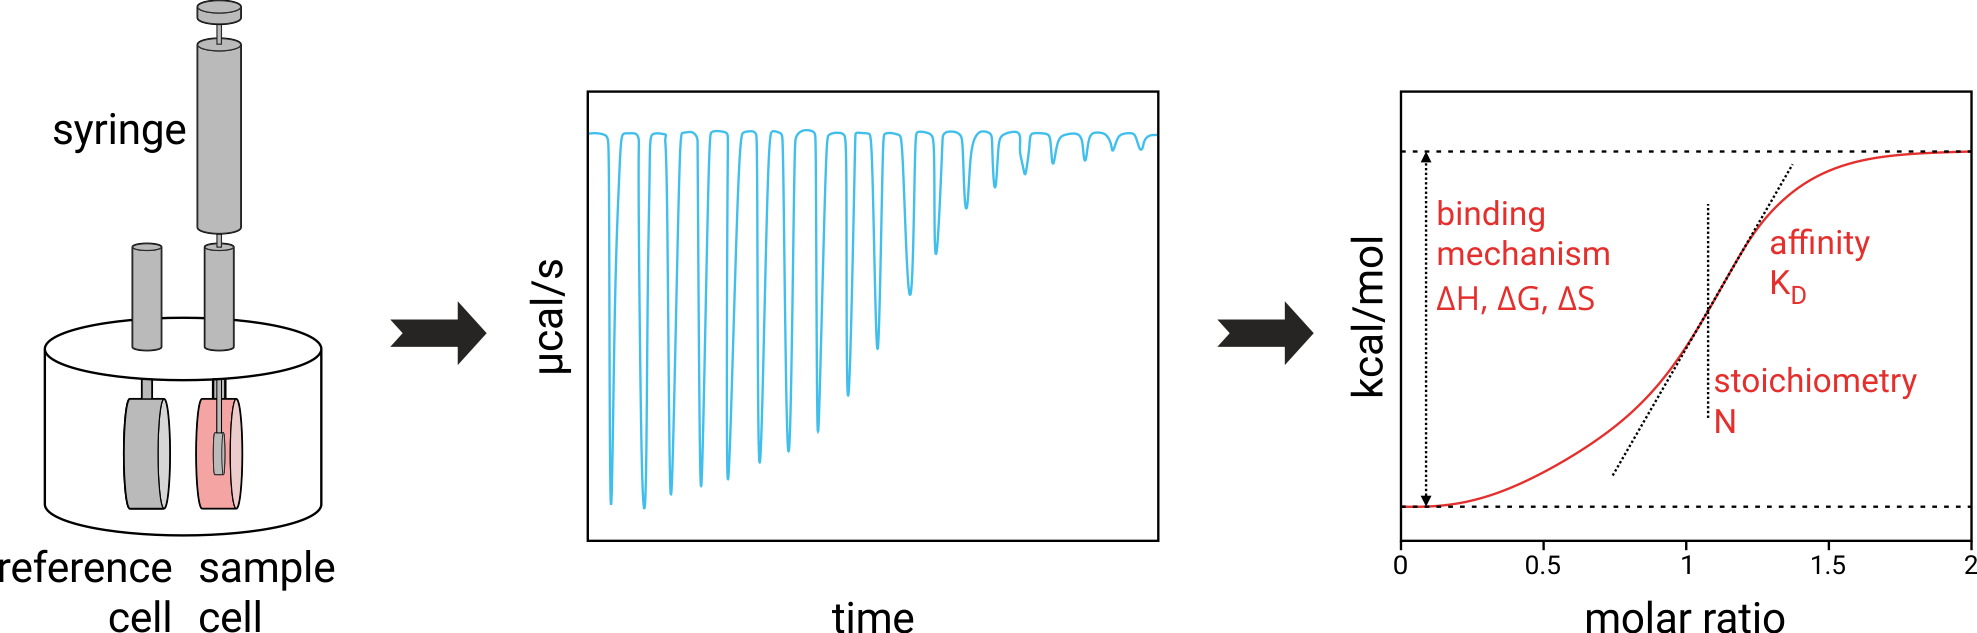
\includegraphics[width=0.8\linewidth]{sources/titration}
	\end{figure}	
	\fcite{tellinghuisen2007optimizing}
	\fcite{wadso2003new}
\end{frame}

\section{Results and Discussion}
\begin{frame}{Temperature sensors calibration}
	\begin{itemize}
		\item A heating ramp was made to calibrate the sensors.
		\item Hg thermometer was used as a reference.
		\item From 10 $^\circ$C to 50 $^\circ$C, steps of 5 $^\circ$C.
		\item Minimum stabilization time of 18 minutes.
	\end{itemize}
	\begin{figure}[h]
		\centering
		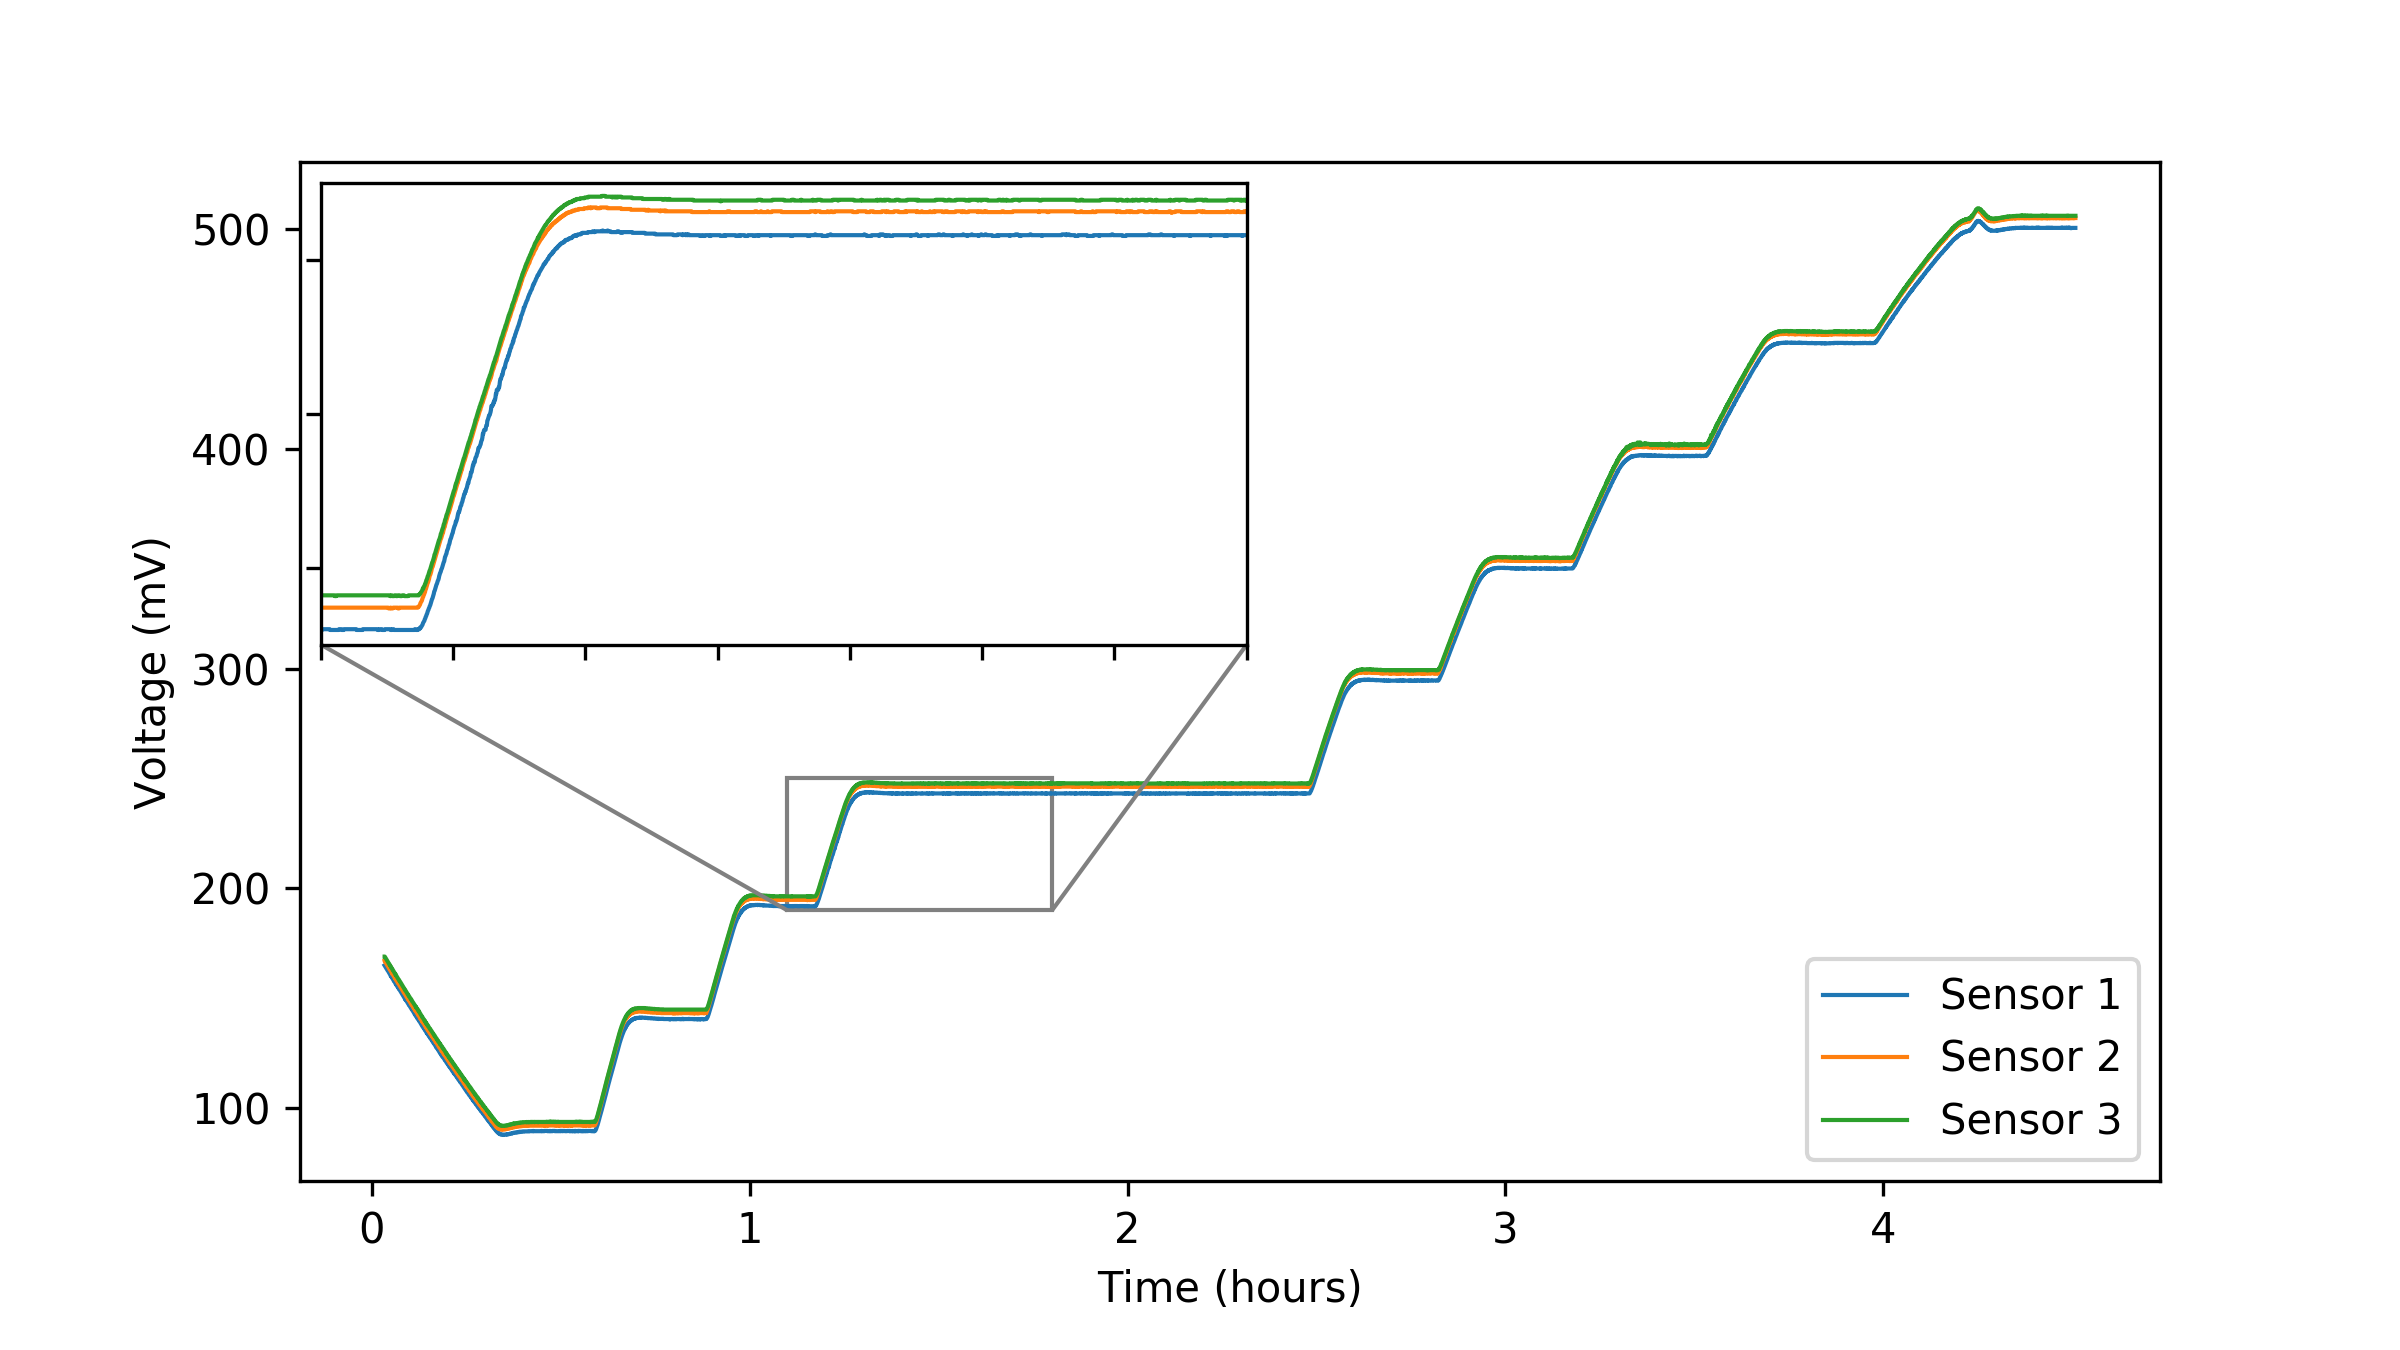
\includegraphics[width=0.9\linewidth]{sources/V-t}
	\end{figure}
\end{frame}

\begin{frame}{Temperature sensors calibration}
	\begin{itemize}
		\item With the use of an algorithm, steady points where found.
		\begin{figure}[h]
			\centering
			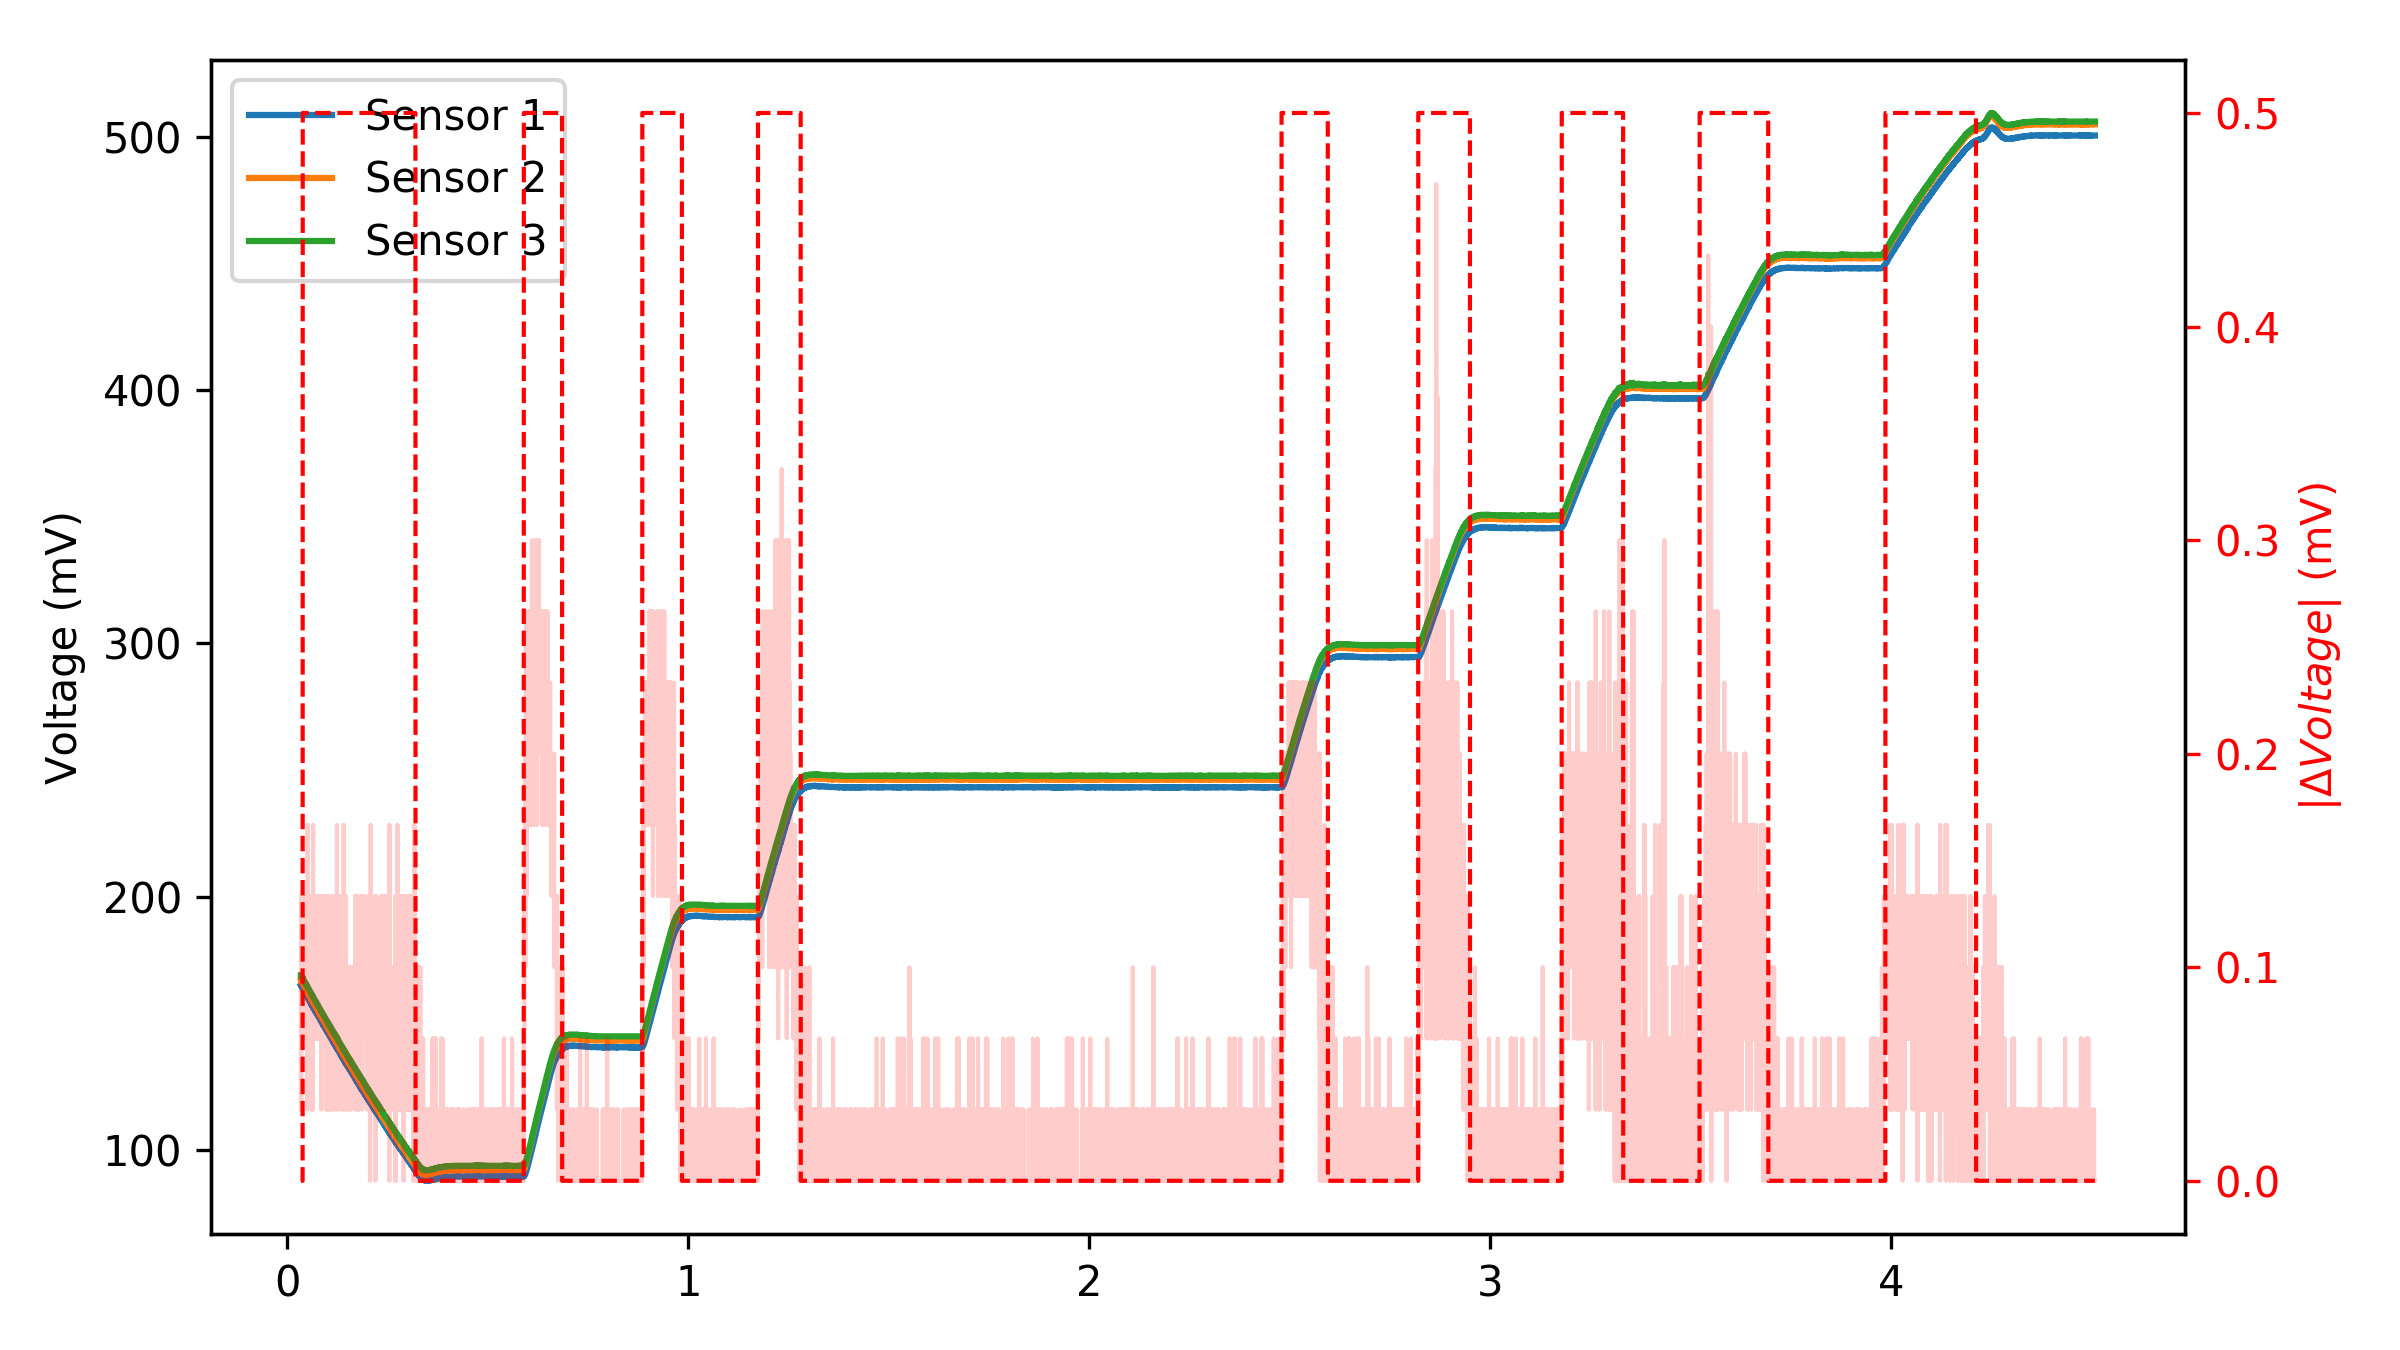
\includegraphics[width=0.5\linewidth]{sources/dV-t}
		\end{figure}
		\item A linear regression was made to find an equivalence between voltage and temperature.
		\begin{figure}[h]
			\centering
			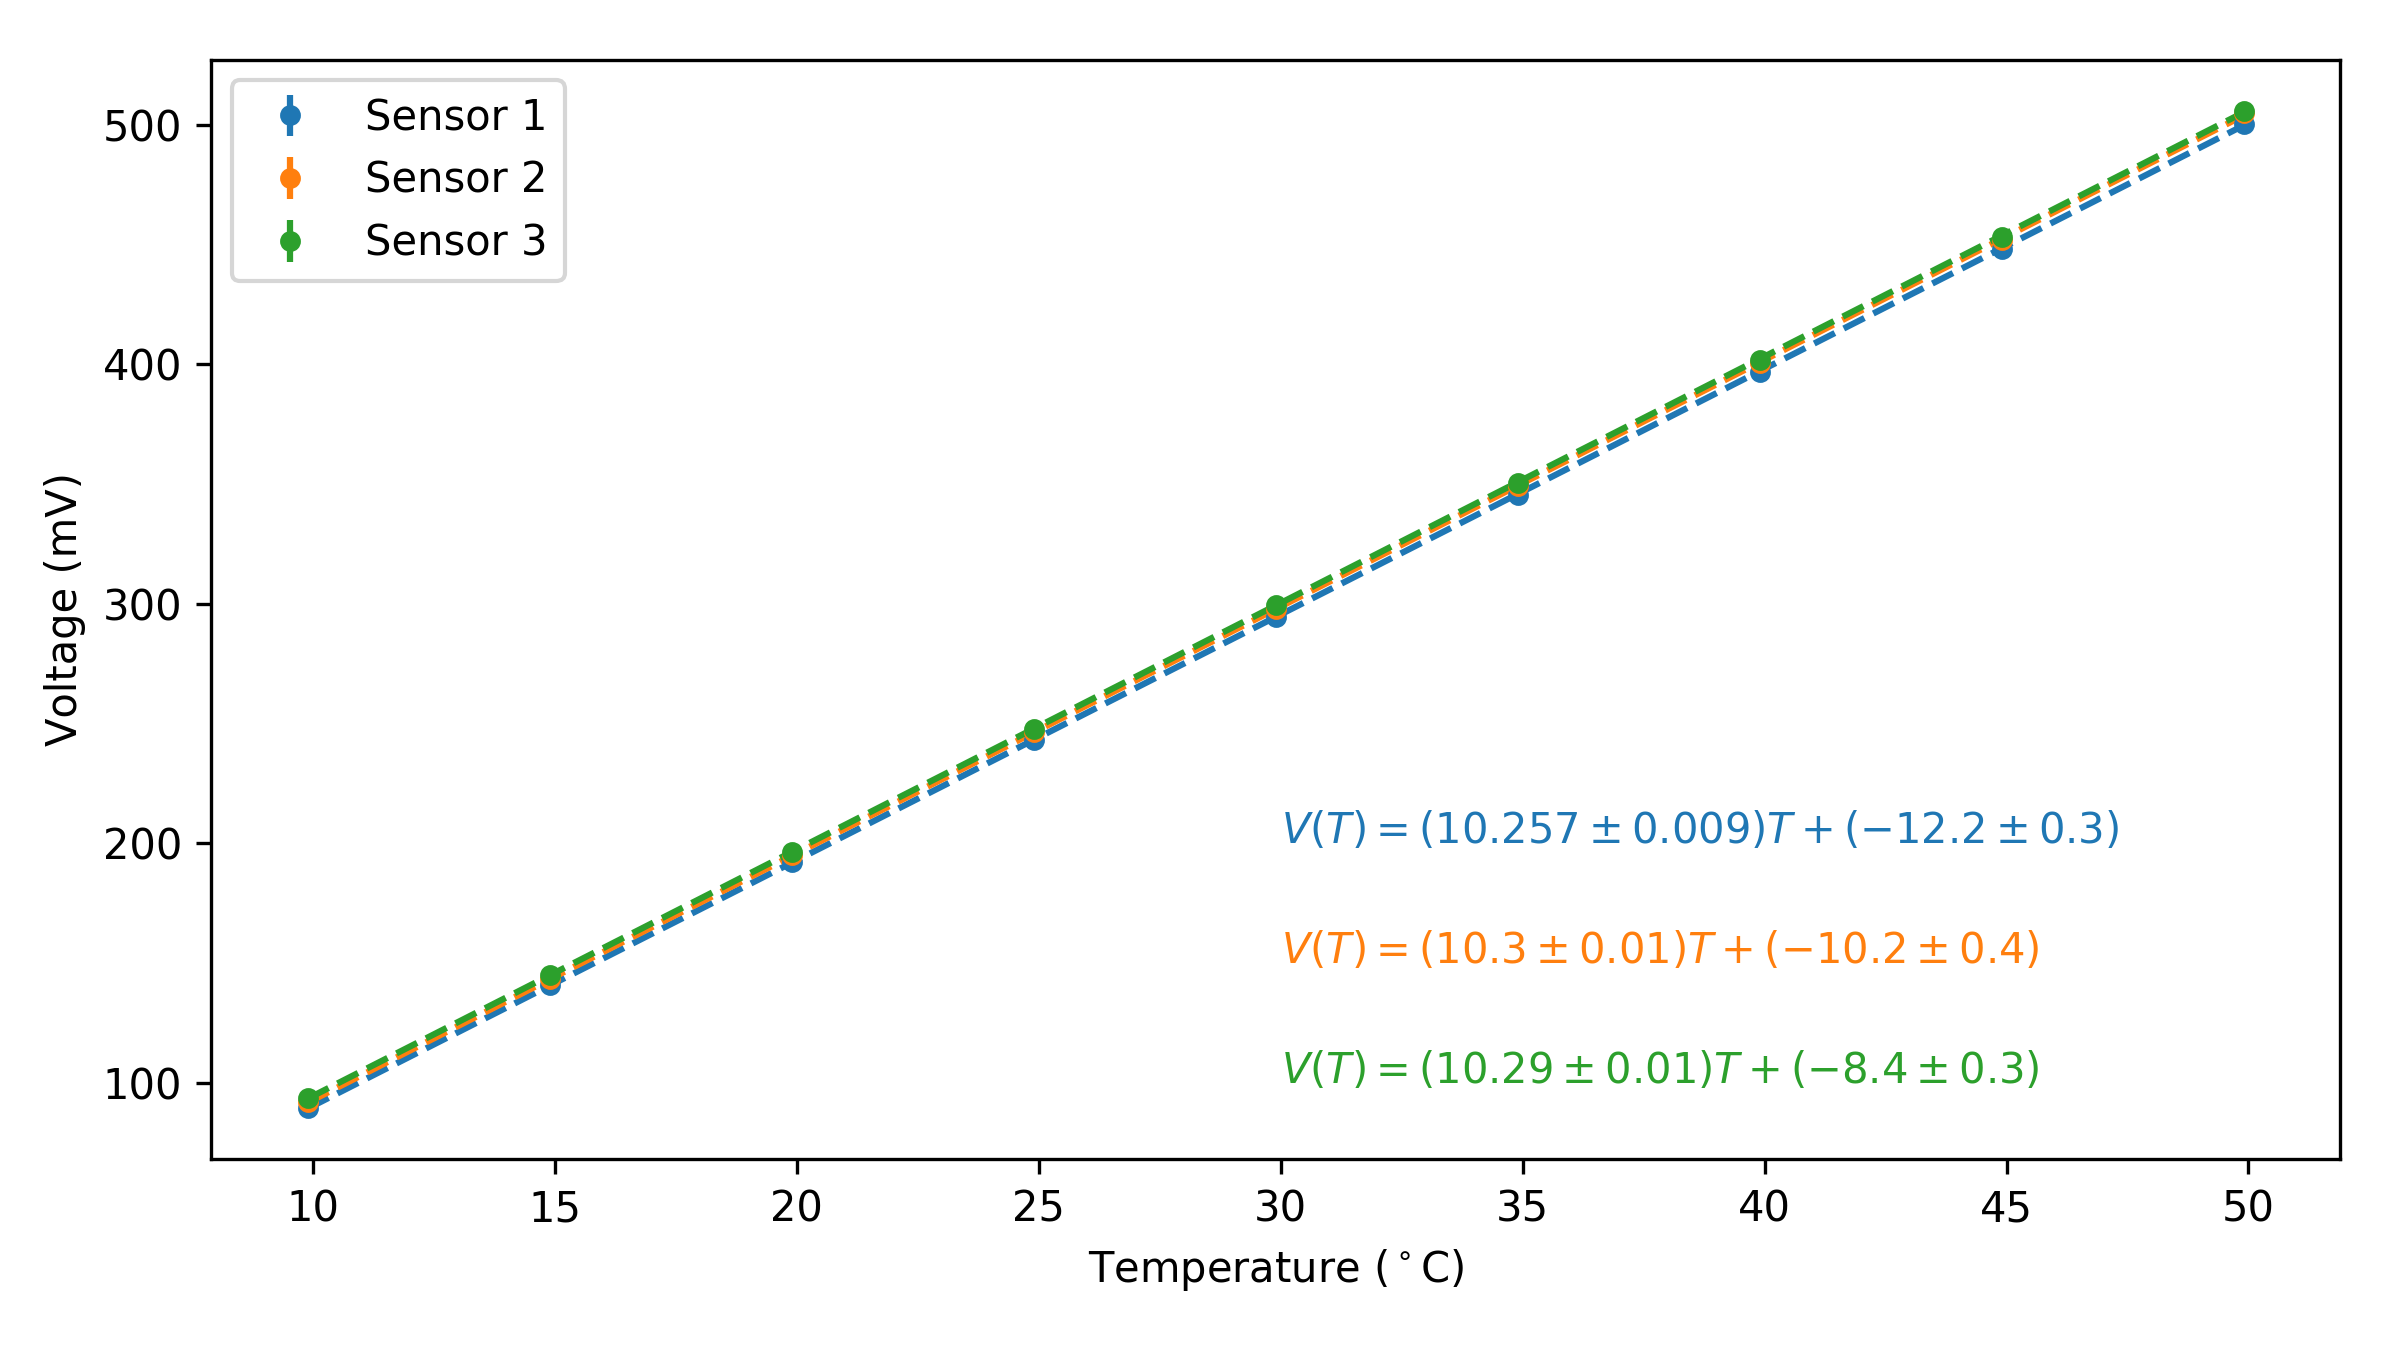
\includegraphics[width=0.6\linewidth]{sources/V-T}
		\end{figure}
	\end{itemize}
\end{frame}

\begin{frame}{Temperature sensors calibration}
	\begin{figure}[h]
		\centering
		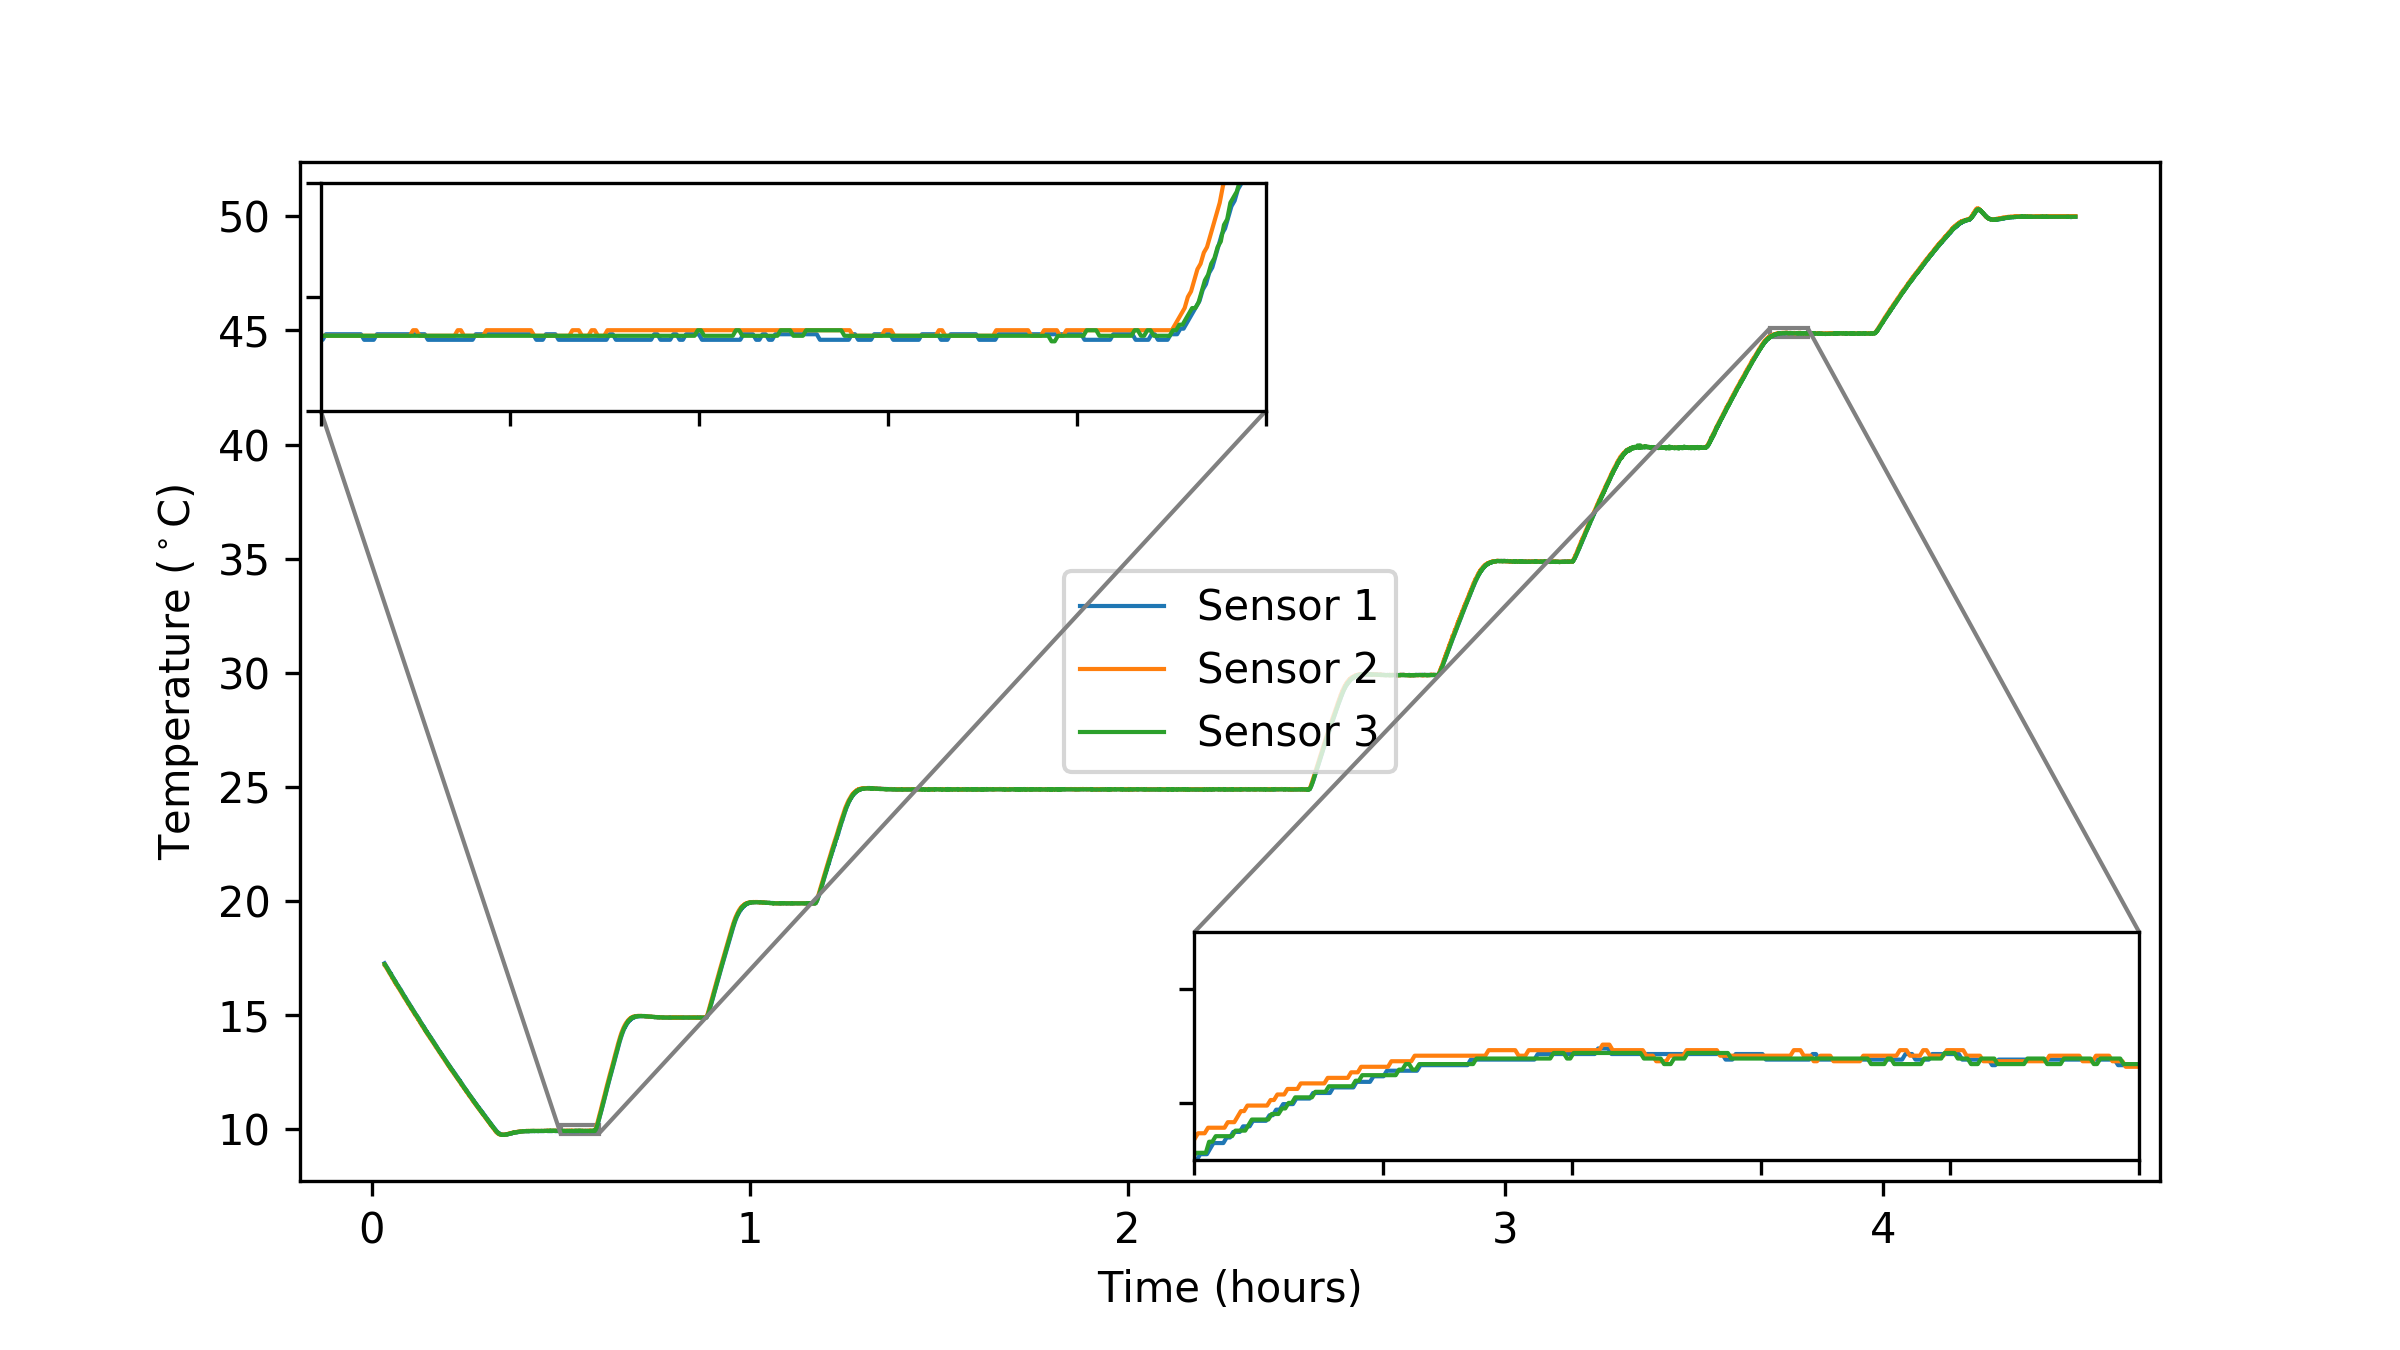
\includegraphics[width=\linewidth]{sources/T-t}
	\end{figure}
\end{frame}

\begin{frame}{Electrical Calibrations}
	\begin{figure}[h]
		\centering
		\begin{tabular}{cc}
			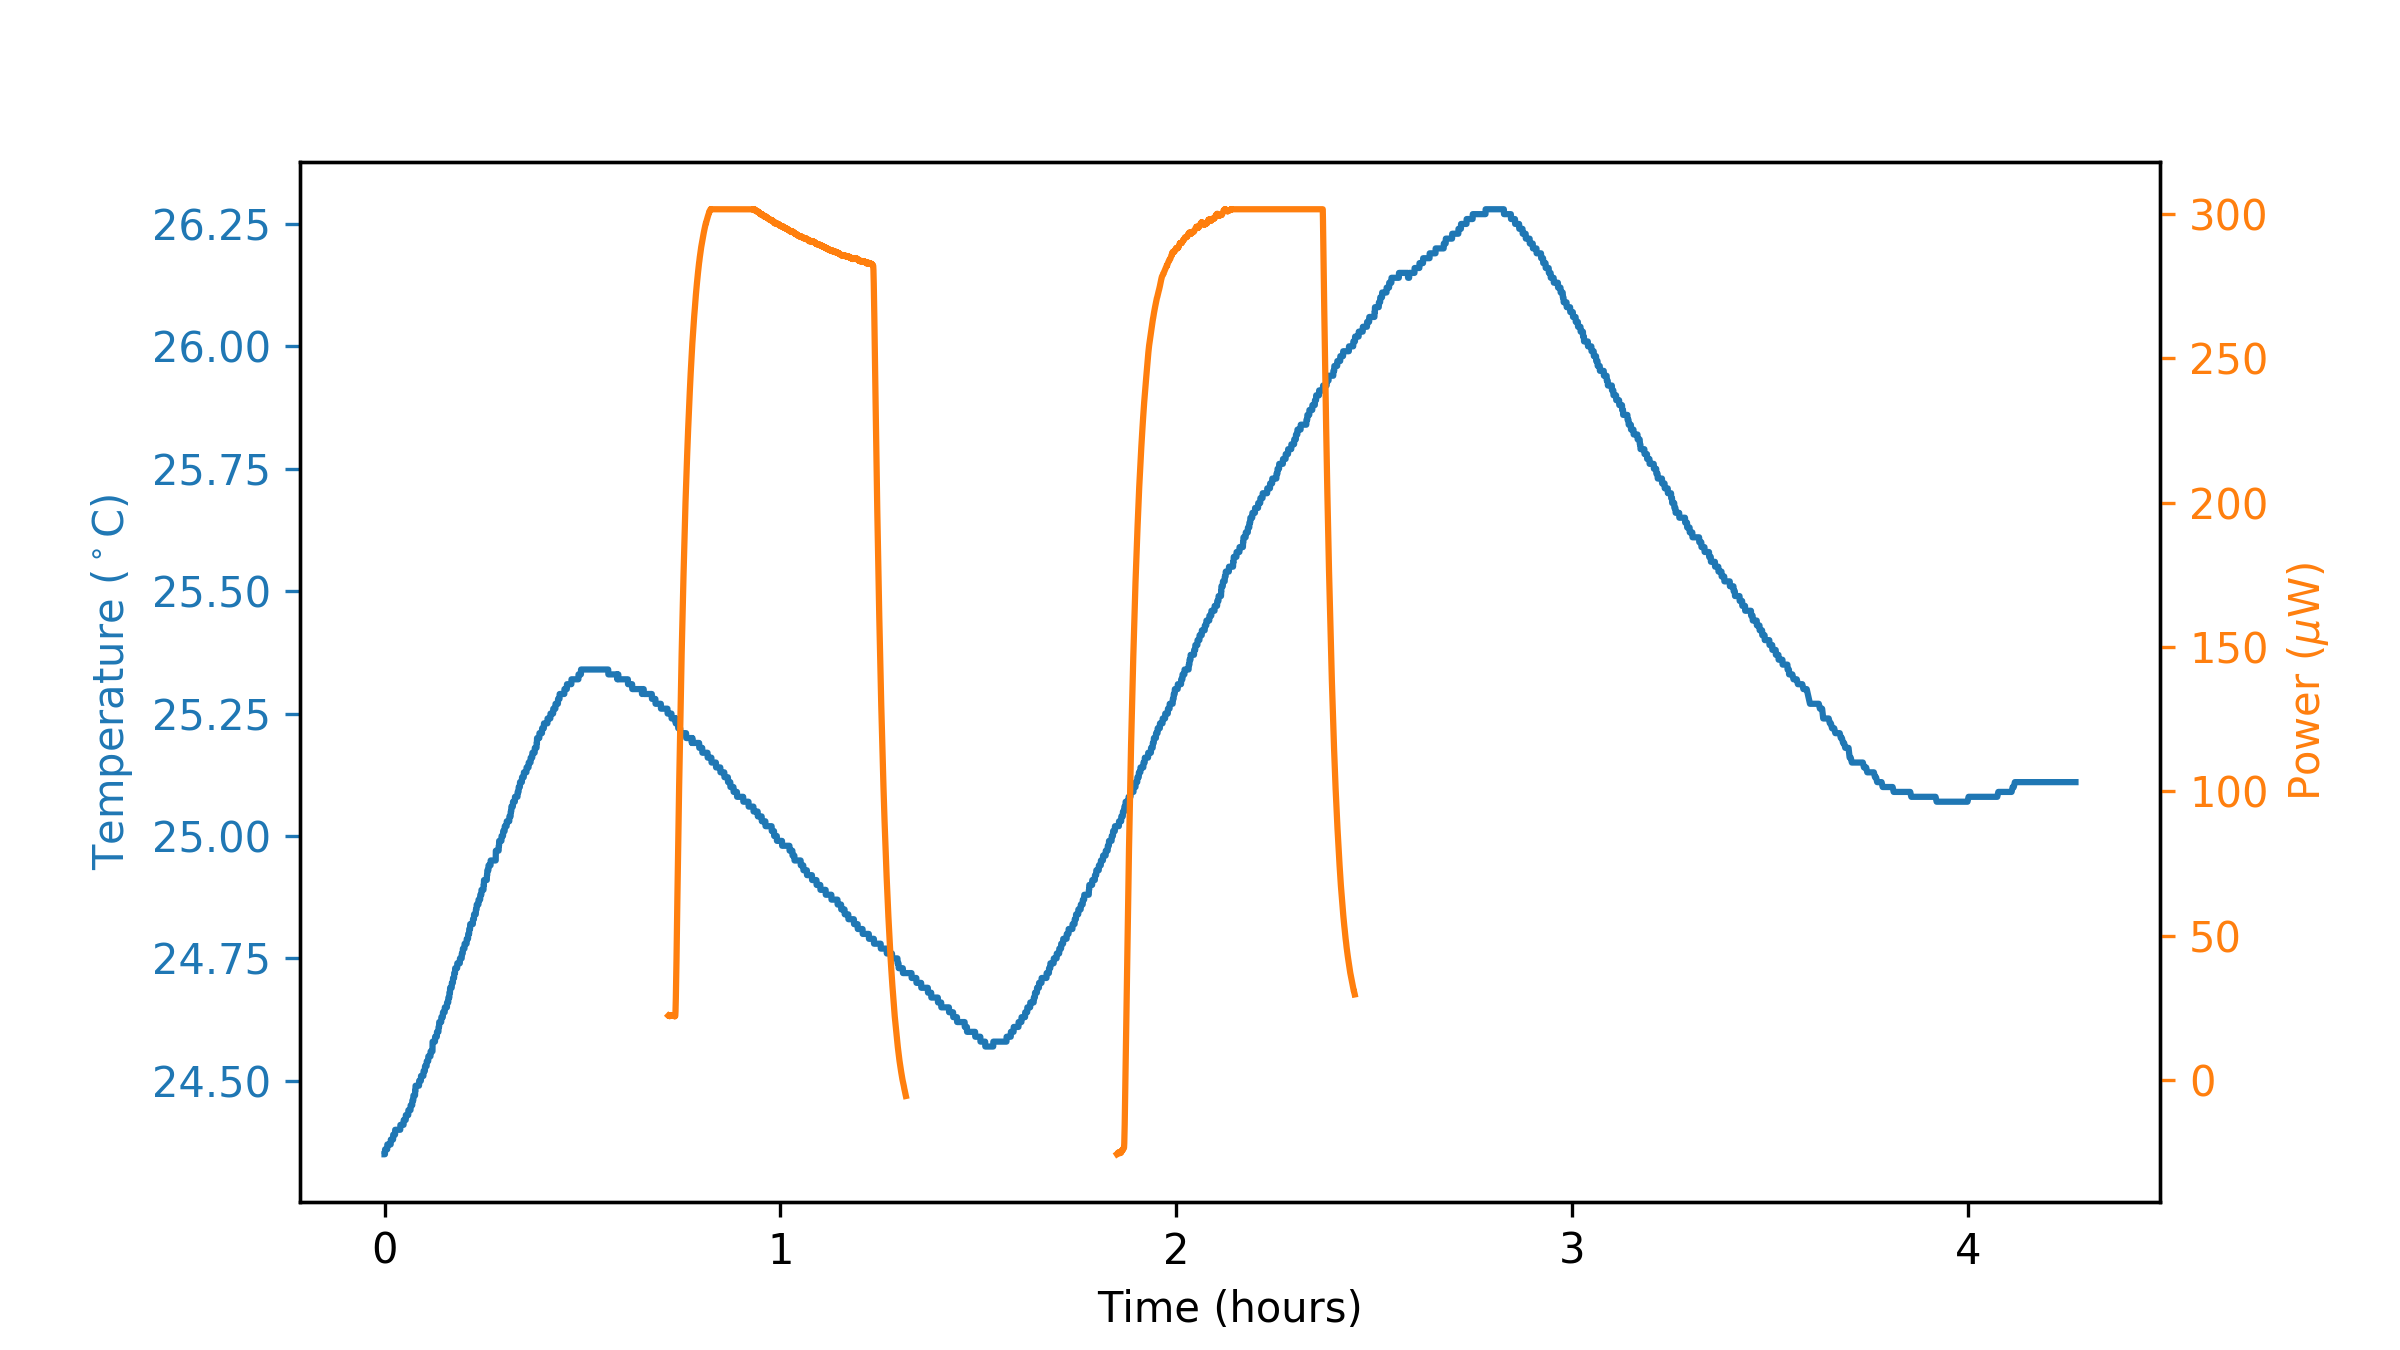
\includegraphics[width=0.49\linewidth]{sources/Cal00-01} & 
			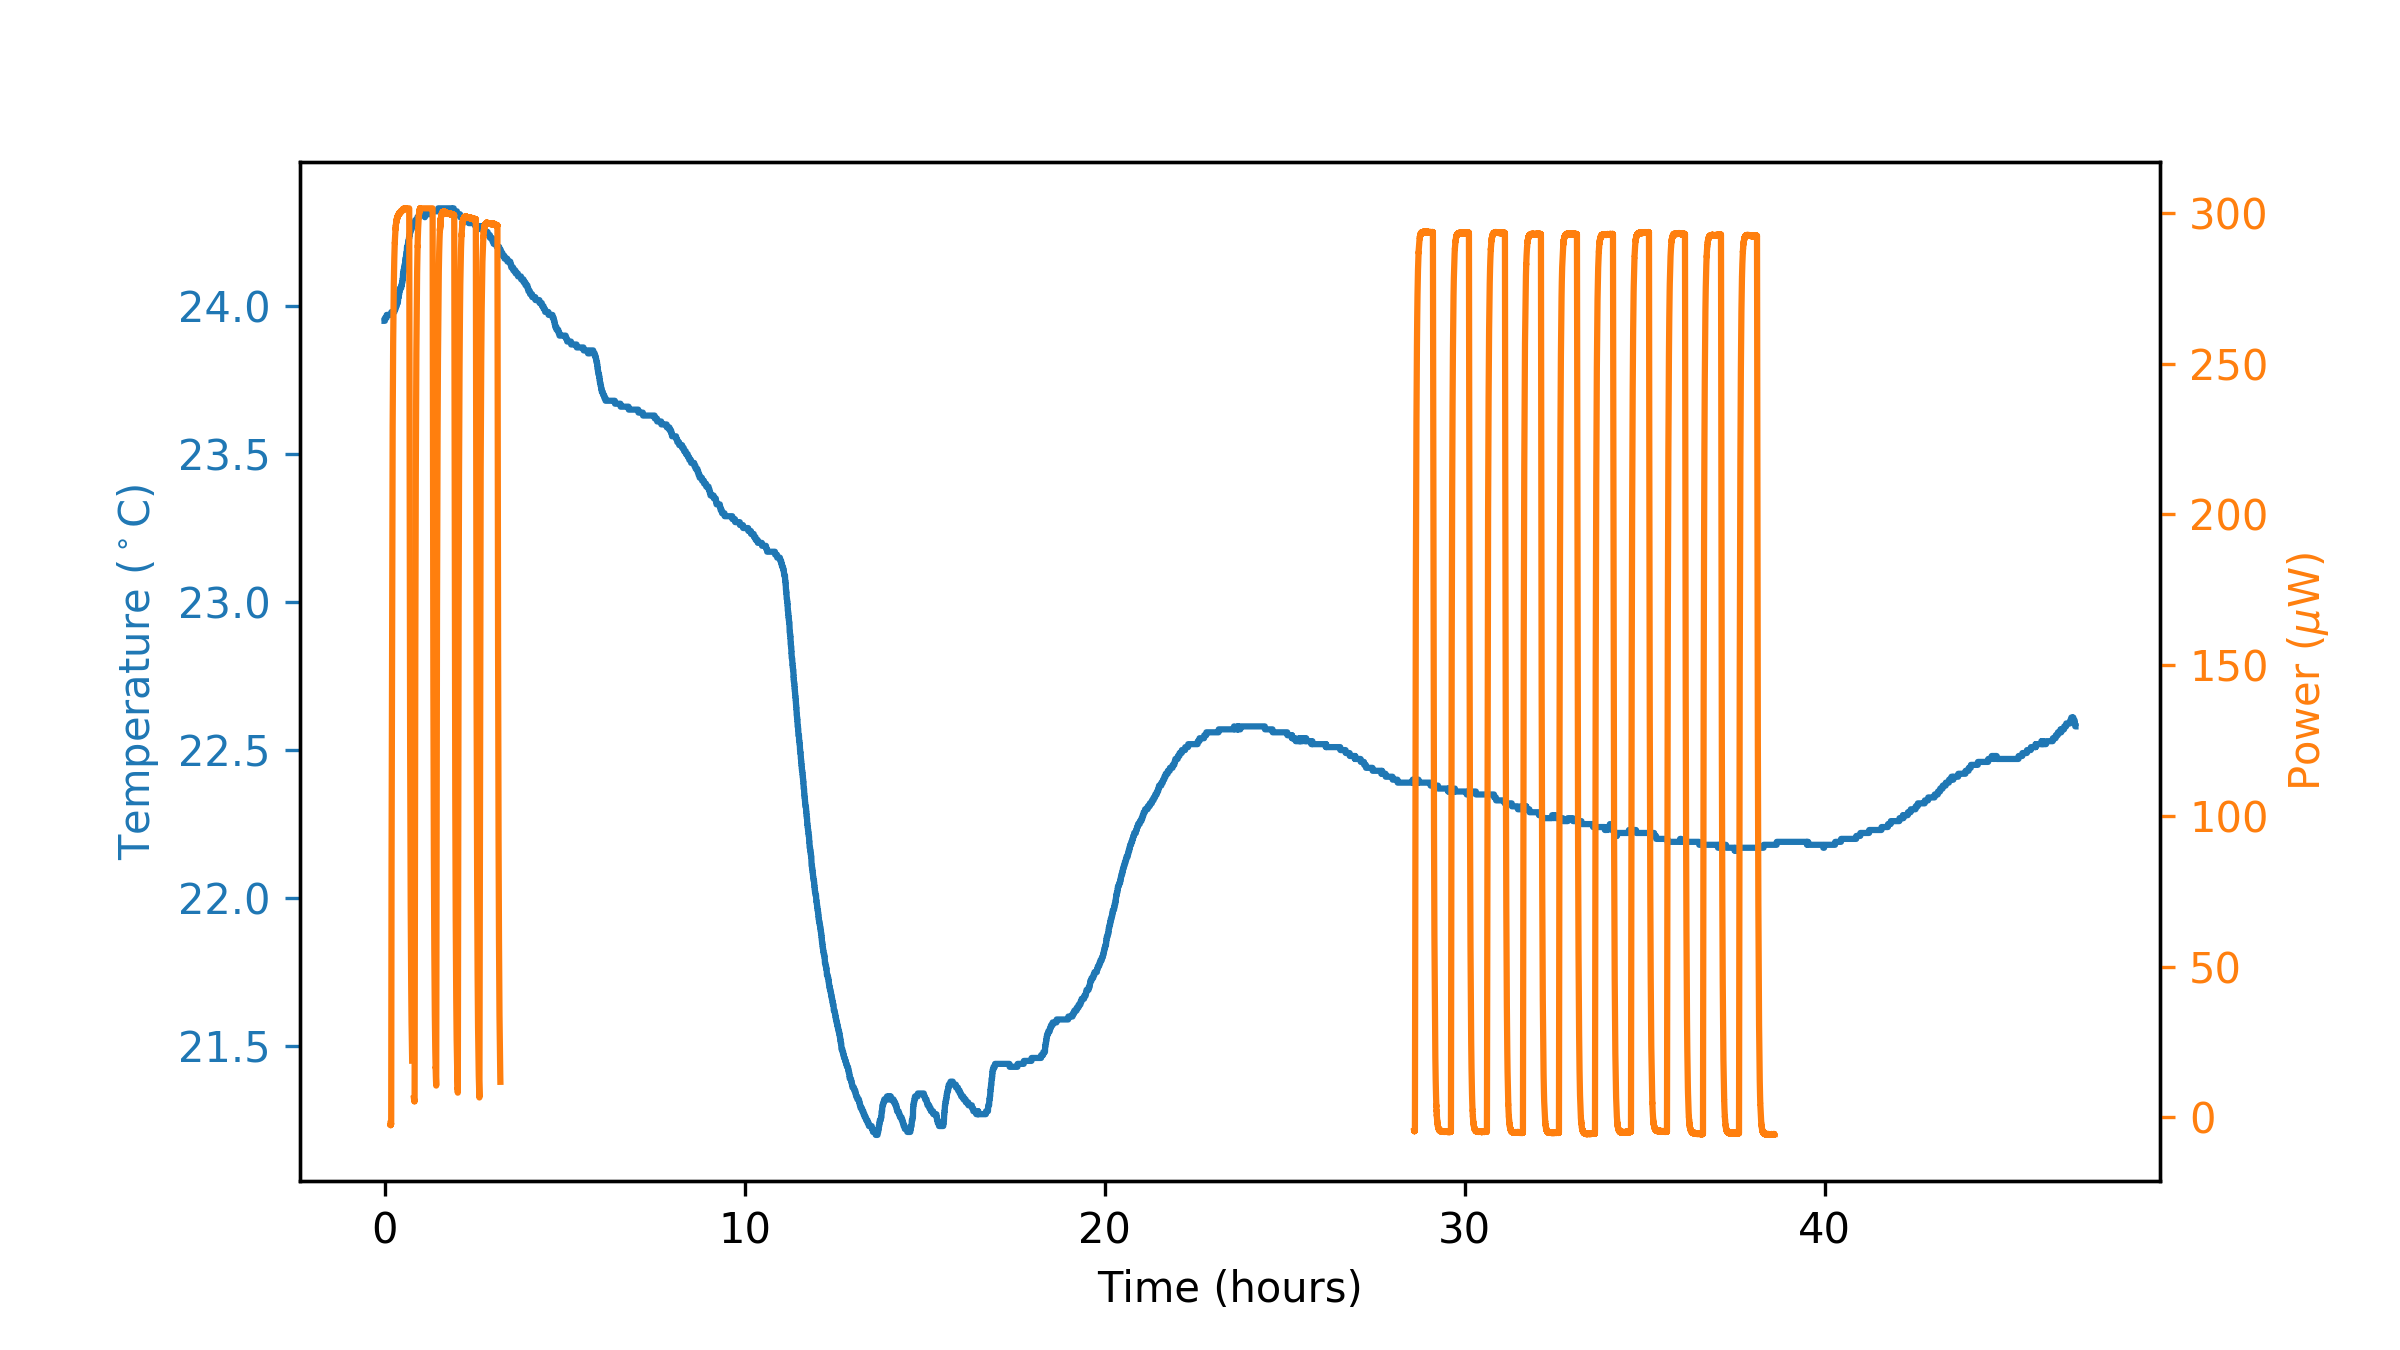
\includegraphics[width=0.49\linewidth]{sources/Calibrations}
		\end{tabular}
		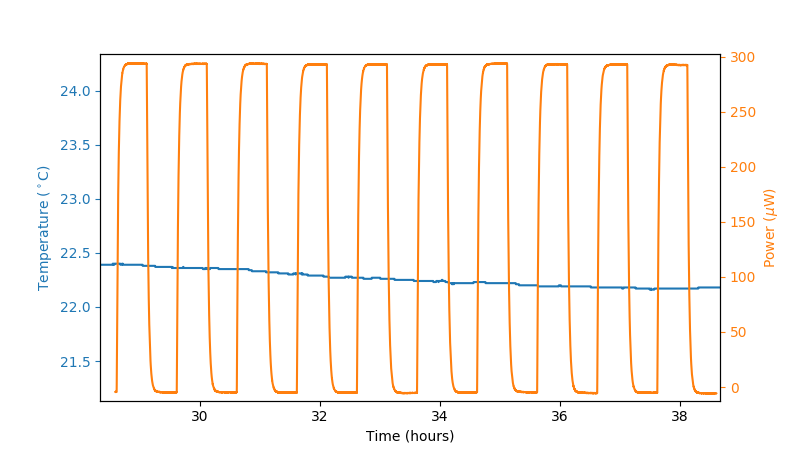
\includegraphics[width=0.70\linewidth]{sources/zCal}
	\end{figure}
\end{frame}

\begin{frame}{Temperature Stability}
	\begin{figure}[h]
		\centering
		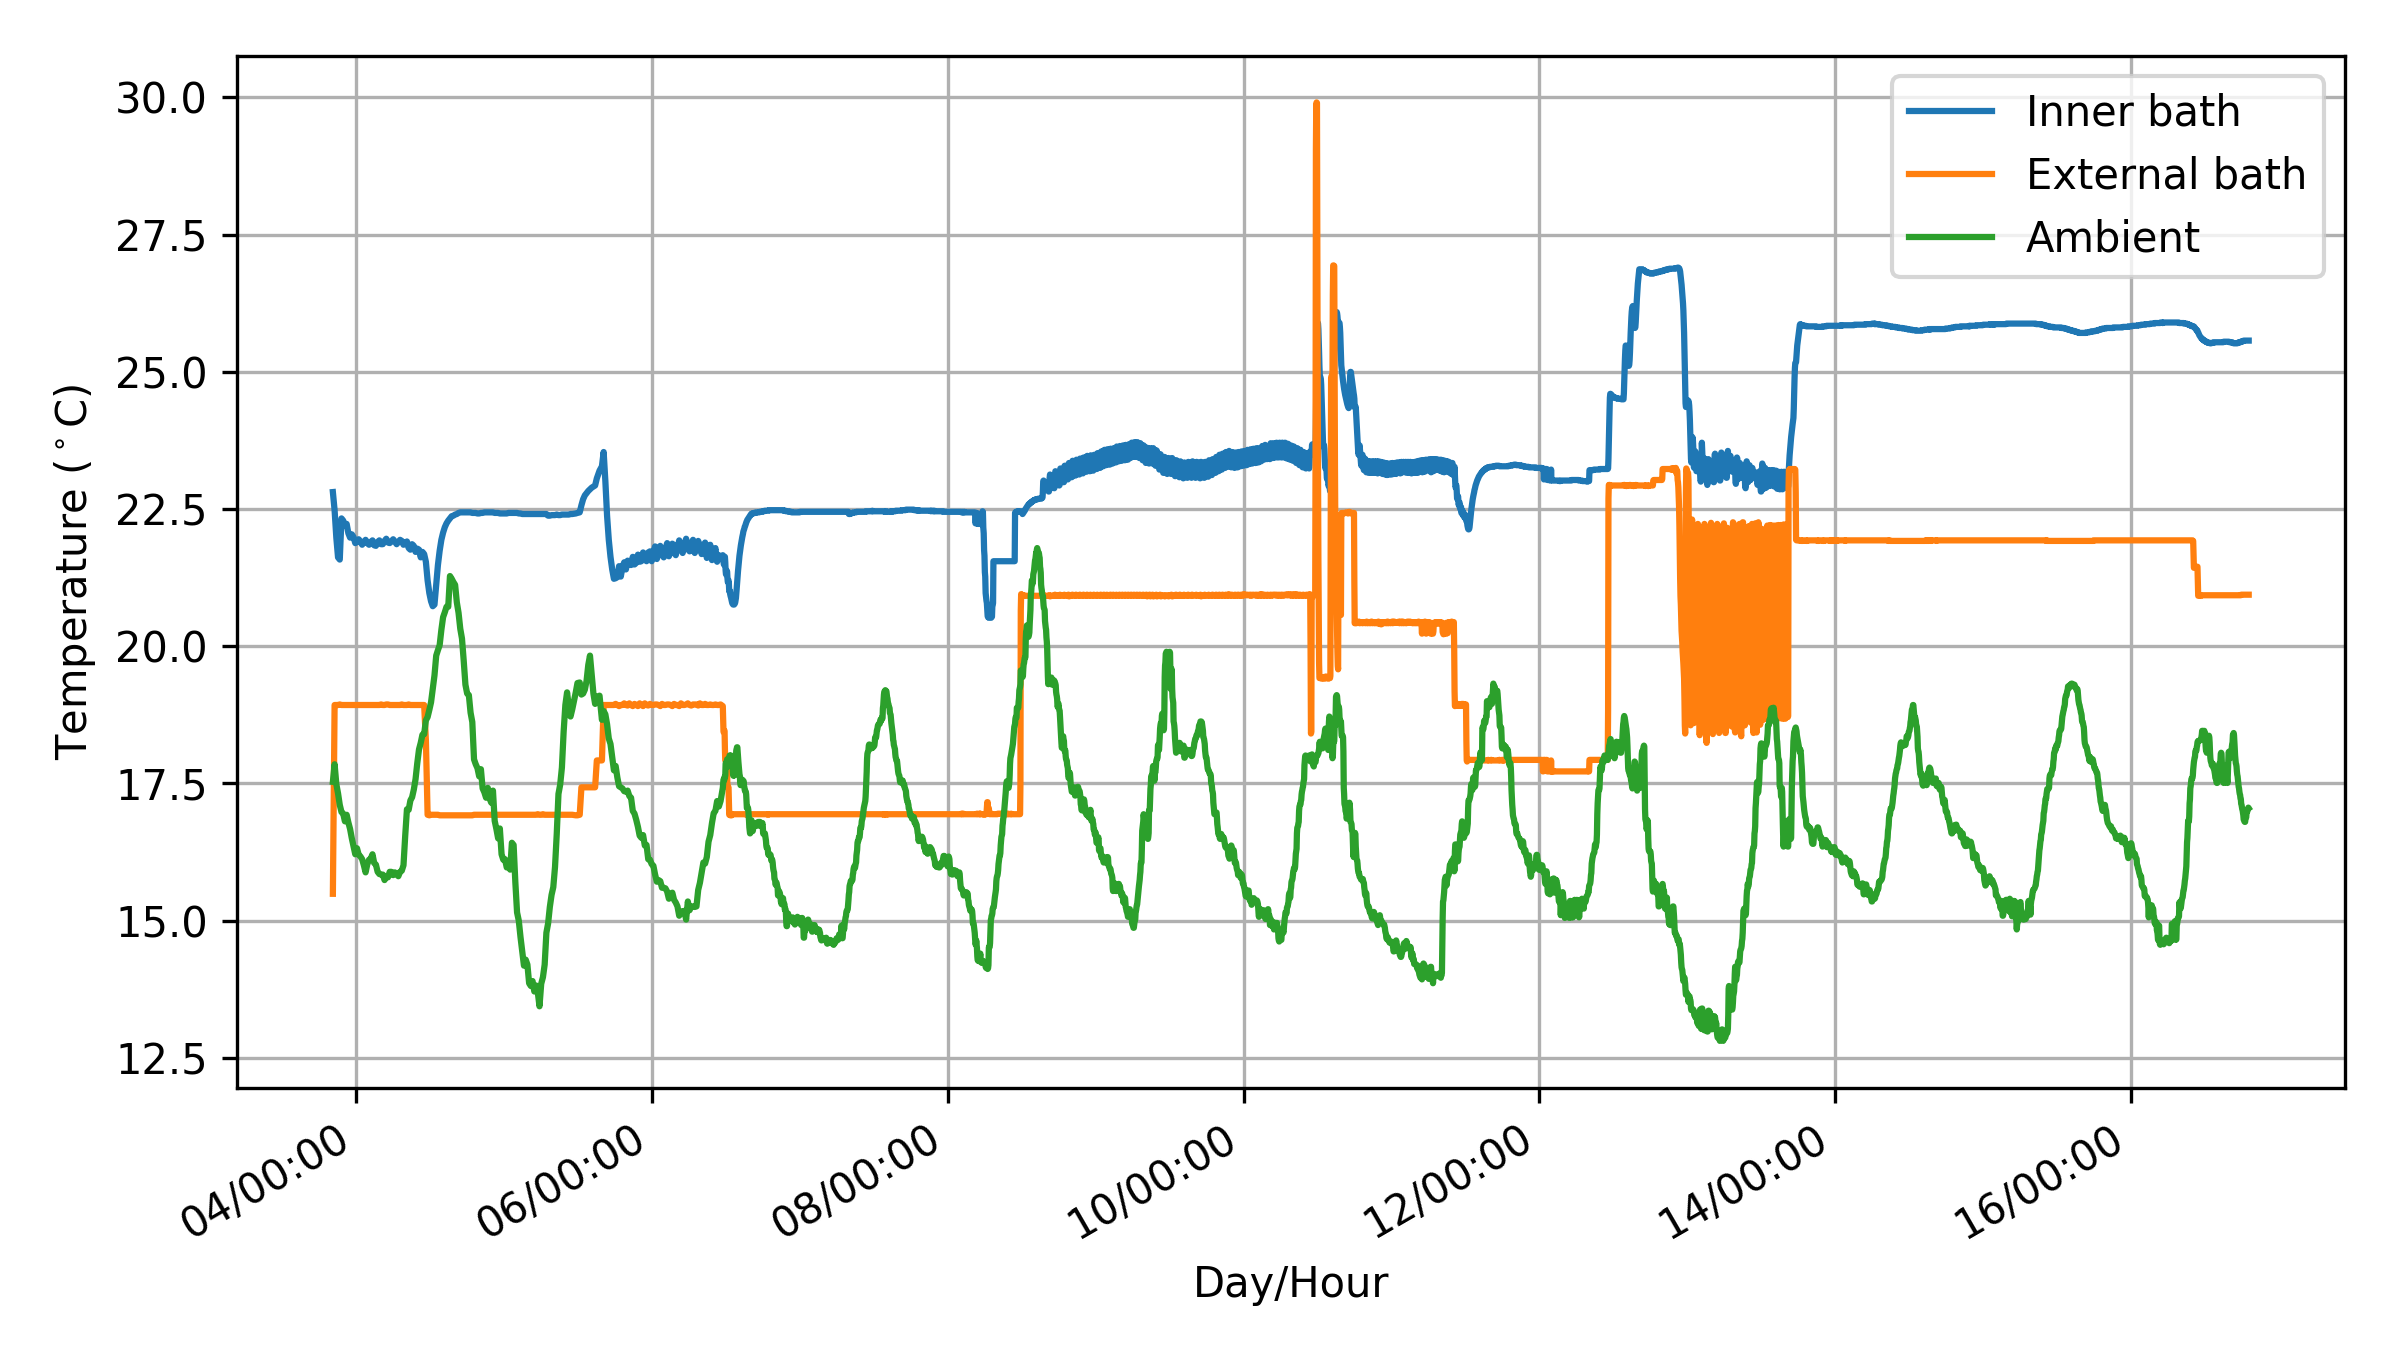
\includegraphics[width=\linewidth]{sources/Stability}
	\end{figure}
\end{frame}

\begin{frame}{Temperature Stability}
	\begin{figure}[h]
		\centering
		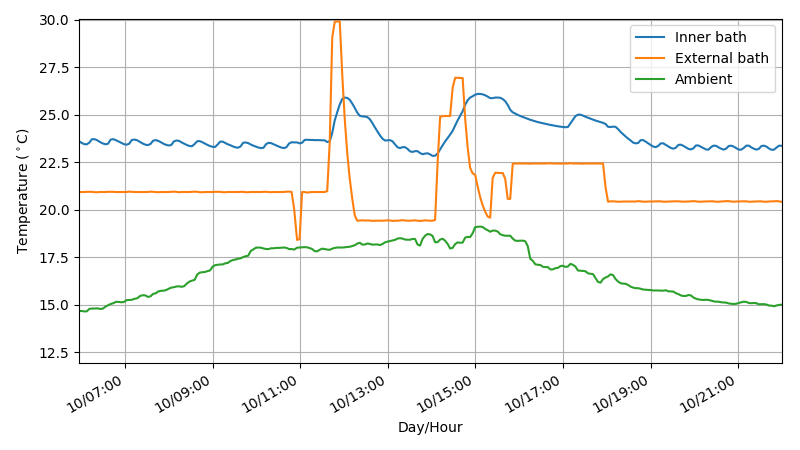
\includegraphics[width=0.6\linewidth]{sources/T1}
		
		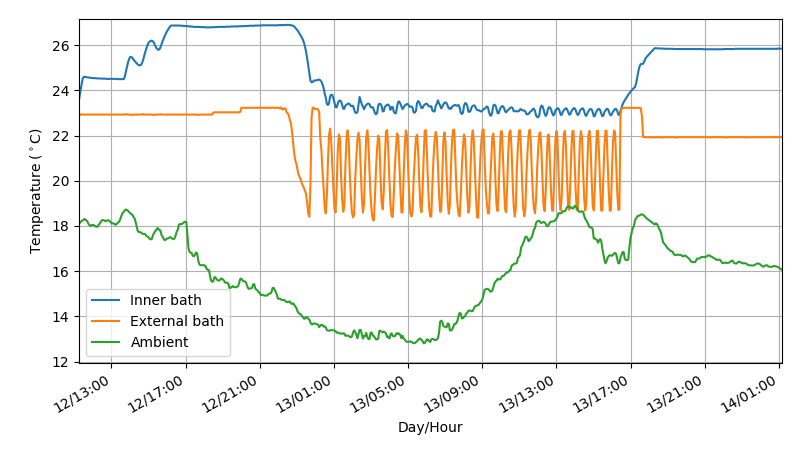
\includegraphics[width=0.6\linewidth]{sources/T2}
	\end{figure}
\end{frame}

\section{Conclusions}
\begin{frame}{Conclusions}
	\begin{enumerate}
		\item \checkmark Carry out the wiring and electrical connections relevant for the operation of the equipment in Colombia.
		\item $\sim$ Controlling the calorimeter temperature.
		\item \checkmark Do an electrical calibration of the calorimeter.
		\item $\times$ Determine the molar enthalpy, Gibbs free energy, entropy, and equilibrium constant, of the complexation of the barium cation with 18-crown-6 ether.
	\end{enumerate}
\end{frame}

\end{document}